\chapter{Phân tích nhiều chiều dữ liệu thang đo định lượng}

Phân tích dữ liệu nhiều chiều là một lĩnh vực quan trọng của thống kê hiện đại, cho phép chúng ta khám phá và hiểu mối quan hệ phức tạp giữa nhiều biến số đồng thời \cite{johnson2007, anderson1984, mardia1979}. Chương này sẽ trình bày các kỹ thuật cơ bản và nâng cao trong phân tích nhiều chiều, từ những khái niệm cơ sở đến các ứng dụng thực tiễn.

\section{Khái niệm cơ bản về dữ liệu nhiều chiều}

\subsection{Vector ngẫu nhiên và phân phối nhiều chiều}
\begin{dn}[Vector ngẫu nhiên]
Vector ngẫu nhiên $p$-chiều là một ánh xạ $\mathbf{X}: \Omega \to \mathbb{R}^p$ được viết dưới dạng
\[
\mathbf{X} = \begin{pmatrix} X_1 \\ X_2 \\ \vdots \\ X_p \end{pmatrix}
\]
trong đó mỗi $X_i$ là một biến ngẫu nhiên.
\end{dn}

\subsection{Vector kỳ vọng và ma trận hiệp phương sai}
\begin{dn}[Vector kỳ vọng]
\[
\boldsymbol{\mu} = \mathbb{E}[\mathbf{X}] = \begin{pmatrix} \mathbb{E}[X_1] \\ \mathbb{E}[X_2] \\ \vdots \\ \mathbb{E}[X_p] \end{pmatrix}
\]
\end{dn}

\begin{dn}[Ma trận hiệp phương sai]
\[
\boldsymbol{\Sigma} = \text{Cov}(\mathbf{X}) = \mathbb{E}[(\mathbf{X} - \boldsymbol{\mu})(\mathbf{X} - \boldsymbol{\mu})^T]
\]
với phần tử thứ $(i,j)$ là $\Sigma_{ij} = \text{Cov}(X_i, X_j)$.
\end{dn}

\begin{tinhchat}[Tính chất của ma trận hiệp phương sai]
\begin{itemize}
    \item $\boldsymbol{\Sigma}$ là ma trận đối xứng: $\boldsymbol{\Sigma} = \boldsymbol{\Sigma}^T$
    \item $\boldsymbol{\Sigma}$ là ma trận nửa xác định dương
    \item Đường chéo chính chứa các phương sai: $\Sigma_{ii} = \text{Var}(X_i)$
\end{itemize}
\end{tinhchat}

\subsection{Phân phối chuẩn nhiều chiều}
\begin{dn}[Phân phối chuẩn nhiều chiều]
Vector ngẫu nhiên $\mathbf{X}$ có phân phối chuẩn nhiều chiều $\mathcal{N}_p(\boldsymbol{\mu}, \boldsymbol{\Sigma})$ nếu có hàm mật độ:
\[
f(\mathbf{x}) = \frac{1}{(2\pi)^{p/2}|\boldsymbol{\Sigma}|^{1/2}} \exp\left(-\frac{1}{2}(\mathbf{x} - \boldsymbol{\mu})^T\boldsymbol{\Sigma}^{-1}(\mathbf{x} - \boldsymbol{\mu})\right)
\]
\end{dn}

\section{Ma trận tương quan và các đặc trưng mô tả}

\subsection{Ma trận tương quan}
\begin{dn}[Ma trận tương quan]
Ma trận tương quan $\mathbf{R}$ có phần tử thứ $(i,j)$ là:
\[
\rho_{ij} = \frac{\text{Cov}(X_i, X_j)}{\sqrt{\text{Var}(X_i)\text{Var}(X_j)}} = \frac{\Sigma_{ij}}{\sqrt{\Sigma_{ii}\Sigma_{jj}}}
\]
\end{dn}

Mối quan hệ giữa ma trận hiệp phương sai và ma trận tương quan:
\[
\boldsymbol{\Sigma} = \mathbf{D}^{1/2} \mathbf{R} \mathbf{D}^{1/2}
\]
trong đó $\mathbf{D} = \text{diag}(\Sigma_{11}, \Sigma_{22}, \ldots, \Sigma_{pp})$.

\subsection{Ước lượng mẫu}
Với mẫu $\mathbf{x}_1, \mathbf{x}_2, \ldots, \mathbf{x}_n$:

\textbf{Vector trung bình mẫu:}
\[
\overline{\mathbf{x}} = \frac{1}{n}\sum_{i=1}^n \mathbf{x}_i
\]

\textbf{Ma trận hiệp phương sai mẫu:}
\[
\mathbf{S} = \frac{1}{n-1}\sum_{i=1}^n (\mathbf{x}_i - \overline{\mathbf{x}})(\mathbf{x}_i - \overline{\mathbf{x}})^T
\]

\textbf{Ma trận tương quan mẫu:}
\[
\mathbf{R} = \mathbf{D}_S^{-1/2} \mathbf{S} \mathbf{D}_S^{-1/2}
\]
với $\mathbf{D}_S = \text{diag}(S_{11}, S_{22}, \ldots, S_{pp})$.

\section{Phân tích thành phần chính (Principal Component Analysis - PCA)}

\subsection{Động lực và ý tưởng cơ bản}
PCA là kỹ thuật giảm chiều dữ liệu bằng cách tìm các hướng có phương sai lớn nhất. Mục tiêu là chuyển đổi dữ liệu gốc $p$-chiều thành không gian mới có chiều thấp hơn mà vẫn giữ được nhiều thông tin nhất.

\subsection{Định nghĩa toán học}
\begin{dn}[Thành phần chính thứ nhất]
Thành phần chính thứ nhất là tổ hợp tuyến tính $Y_1 = \mathbf{a}_1^T\mathbf{X}$ sao cho:
\begin{itemize}
    \item $\text{Var}(Y_1) = \mathbf{a}_1^T\boldsymbol{\Sigma}\mathbf{a}_1$ đạt giá trị lớn nhất
    \item Ràng buộc: $\|\mathbf{a}_1\| = 1$
\end{itemize}
\end{dn}

\begin{dl}[Nghiệm của bài toán PCA]
Các thành phần chính được xác định thông qua phân tích trị riêng của ma trận hiệp phương sai:
\[
\boldsymbol{\Sigma}\mathbf{a}_i = \lambda_i\mathbf{a}_i, \quad i = 1, 2, \ldots, p
\]
với $\lambda_1 \geq \lambda_2 \geq \cdots \geq \lambda_p \geq 0$ và $\|\mathbf{a}_i\| = 1$.
\end{dl}

\subsection{Tính chất quan trọng}
\begin{tinhchat}[Tính chất của PCA]
\begin{itemize}
    \item Phương sai của thành phần chính thứ $i$: $\text{Var}(Y_i) = \lambda_i$
    \item Tổng phương sai được bảo toàn: $\sum_{i=1}^p \lambda_i = \sum_{i=1}^p \text{Var}(X_i)$
    \item Các thành phần chính không tương quan: $\text{Cov}(Y_i, Y_j) = 0$ với $i \neq j$
    \item Tỷ lệ phương sai được giải thích bởi $k$ thành phần đầu: $\frac{\sum_{i=1}^k \lambda_i}{\sum_{i=1}^p \lambda_i}$
\end{itemize}
\end{tinhchat}

\subsection{Thuật toán thực hiện PCA}
\begin{enumerate}
    \item \textbf{Chuẩn hóa dữ liệu}: Chuyển về dạng $Z$-score nếu cần
    \item \textbf{Tính ma trận hiệp phương sai} (hoặc tương quan)
    \item \textbf{Phân tích trị riêng}: Tìm $\lambda_i$ và $\mathbf{a}_i$
    \item \textbf{Sắp xếp}: Theo thứ tự giảm dần của $\lambda_i$
    \item \textbf{Chọn số thành phần}: Dựa trên tiêu chí phù hợp
    \item \textbf{Chuyển đổi dữ liệu}: $\mathbf{Y} = \mathbf{A}^T\mathbf{X}$
\end{enumerate}

\subsection{Tiêu chí lựa chọn số thành phần}
\subsubsection*{Tiêu chí Kaiser}
Giữ lại các thành phần có $\lambda_i > 1$ (khi sử dụng ma trận tương quan).

\subsubsection*{Tiêu chí phần trăm phương sai}
Chọn $k$ sao cho $\frac{\sum_{i=1}^k \lambda_i}{\sum_{i=1}^p \lambda_i} \geq 0.80$ (hoặc 0.85, 0.90).

\subsubsection*{Scree plot}
Vẽ đồ thị $\lambda_i$ theo $i$ và tìm "điểm khuỷu" (elbow point).

\section{Phân tích nhân tố (Factor Analysis)}

\subsection{Mô hình nhân tố}
\begin{dn}[Mô hình nhân tố]
Mô hình nhân tố biểu diễn vector quan sát $\mathbf{X}$ dưới dạng:
\[
\mathbf{X} = \boldsymbol{\mu} + \mathbf{L}\mathbf{F} + \boldsymbol{\epsilon}
\]
trong đó:
\begin{itemize}
    \item $\mathbf{F}$ là vector nhân tố chung $(m \times 1)$ với $m < p$
    \item $\mathbf{L}$ là ma trận tải nhân tố $(p \times m)$
    \item $\boldsymbol{\epsilon}$ là vector sai số cụ thể $(p \times 1)$
\end{itemize}
\end{dn}

\subsection{Giả định của mô hình}
\begin{itemize}
    \item $\mathbb{E}[\mathbf{F}] = \mathbf{0}$ và $\text{Cov}(\mathbf{F}) = \mathbf{I}_m$
    \item $\mathbb{E}[\boldsymbol{\epsilon}] = \mathbf{0}$ và $\text{Cov}(\boldsymbol{\epsilon}) = \boldsymbol{\Psi}$ (ma trận chéo)
    \item $\text{Cov}(\mathbf{F}, \boldsymbol{\epsilon}) = \mathbf{0}$
\end{itemize}

\subsection{Phân tích ma trận hiệp phương sai}
Từ mô hình nhân tố, ta có:
\[
\boldsymbol{\Sigma} = \mathbf{L}\mathbf{L}^T + \boldsymbol{\Psi}
\]

\textbf{Phương sai chung (communality):} $h_i^2 = \sum_{j=1}^m L_{ij}^2$

\textbf{Phương sai cụ thể (specific variance):} $\psi_i = \Sigma_{ii} - h_i^2$

\subsection{Phương pháp ước lượng}
\subsubsection*{Phương pháp thành phần chính}
Sử dụng $m$ thành phần chính đầu tiên để ước lượng ma trận tải:
\[
\hat{\mathbf{L}} = \mathbf{A}_m\boldsymbol{\Lambda}_m^{1/2}
\]
với $\mathbf{A}_m$ chứa $m$ vector riêng đầu và $\boldsymbol{\Lambda}_m = \text{diag}(\lambda_1, \ldots, \lambda_m)$.

\subsubsection*{Phương pháp maximum likelihood}
Tối đa hóa hàm likelihood dưới giả định phân phối chuẩn.

\subsection{Xoay nhân tố (Factor Rotation)}
Mục đích: Tìm ma trận tải dễ giải thích hơn thông qua phép xoay.

\subsubsection*{Xoay Varimax}
Tối đa hóa tổng phương sai của bình phương các tải trong mỗi nhân tố:
\[
V = \sum_{j=1}^m \left[\sum_{i=1}^p L_{ij}^4 - \frac{1}{p}\left(\sum_{i=1}^p L_{ij}^2\right)^2\right]
\]

\subsubsection*{Xoay Promax}
Cho phép các nhân tố tương quan với nhau (oblique rotation).

\section{Áp dụng thuật toán trên R}

Bộ dữ liệu nghiên cứu được thu thập thông qua phiếu khảo sát dành cho giảng viên, chuyên viên, học viên cao học và sinh viên Trường Đại học Cần Thơ, nhằm đánh giá toàn diện mức độ cần thiết, hiệu quả, sự hài lòng và mức độ quan tâm đối với các hoạt động dịch vụ thông tin thư viện tại Trung tâm Học liệu. Phiếu khảo sát bao gồm nhiều nhóm tiêu chí liên quan đến:
\begin{itemize}
    \item Mục đích và vai trò của hoạt động dịch vụ thông tin thư viện.
    \item Các phương pháp triển khai hoạt động dịch vụ.
    \item Mức độ hài lòng và tần suất sử dụng các loại hình dịch vụ.
    \item Mức độ quan tâm của các nhóm đối tượng thụ hưởng.
    \item Điều kiện cơ sở vật chất, hạ tầng và hỗ trợ thông tin.
    \item Tầm quan trọng của công tác quản lý dịch vụ.
\end{itemize}

Các câu hỏi được xây dựng theo thang đo Likert nhiều mức, từ ``Rất cần thiết'' đến ``Không cần thiết'' hoặc từ ``Rất hài lòng'' đến ``Rất không hài lòng'', cho phép định lượng thái độ và nhận thức của người trả lời.

Bộ dữ liệu sau khi thu thập, xử lý được lưu lại với dạng bảng hỏi gồm 60 biến trong excel. Bên dưới minh họa một vài biến trong dữ liệu như sau:
\begin{figure}[h!]
    \centering
    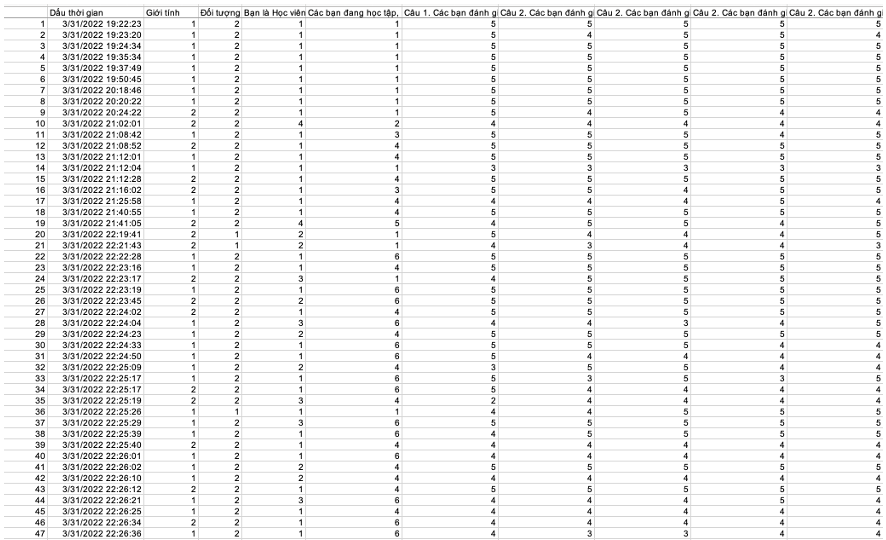
\includegraphics[width=\textwidth]{../../assets/images/SP19.png}
    \caption{Minh họa dữ liệu gốc với 60 biến}
    \label{fig:original_data}
\end{figure}

Với bộ dữ liệu này, tiến hành xáo trộn. Khi đó, chúng tôi thu được dữ liệu khác với cấu trúc ban đầu như sau:
\begin{figure}[h!]
    \centering
    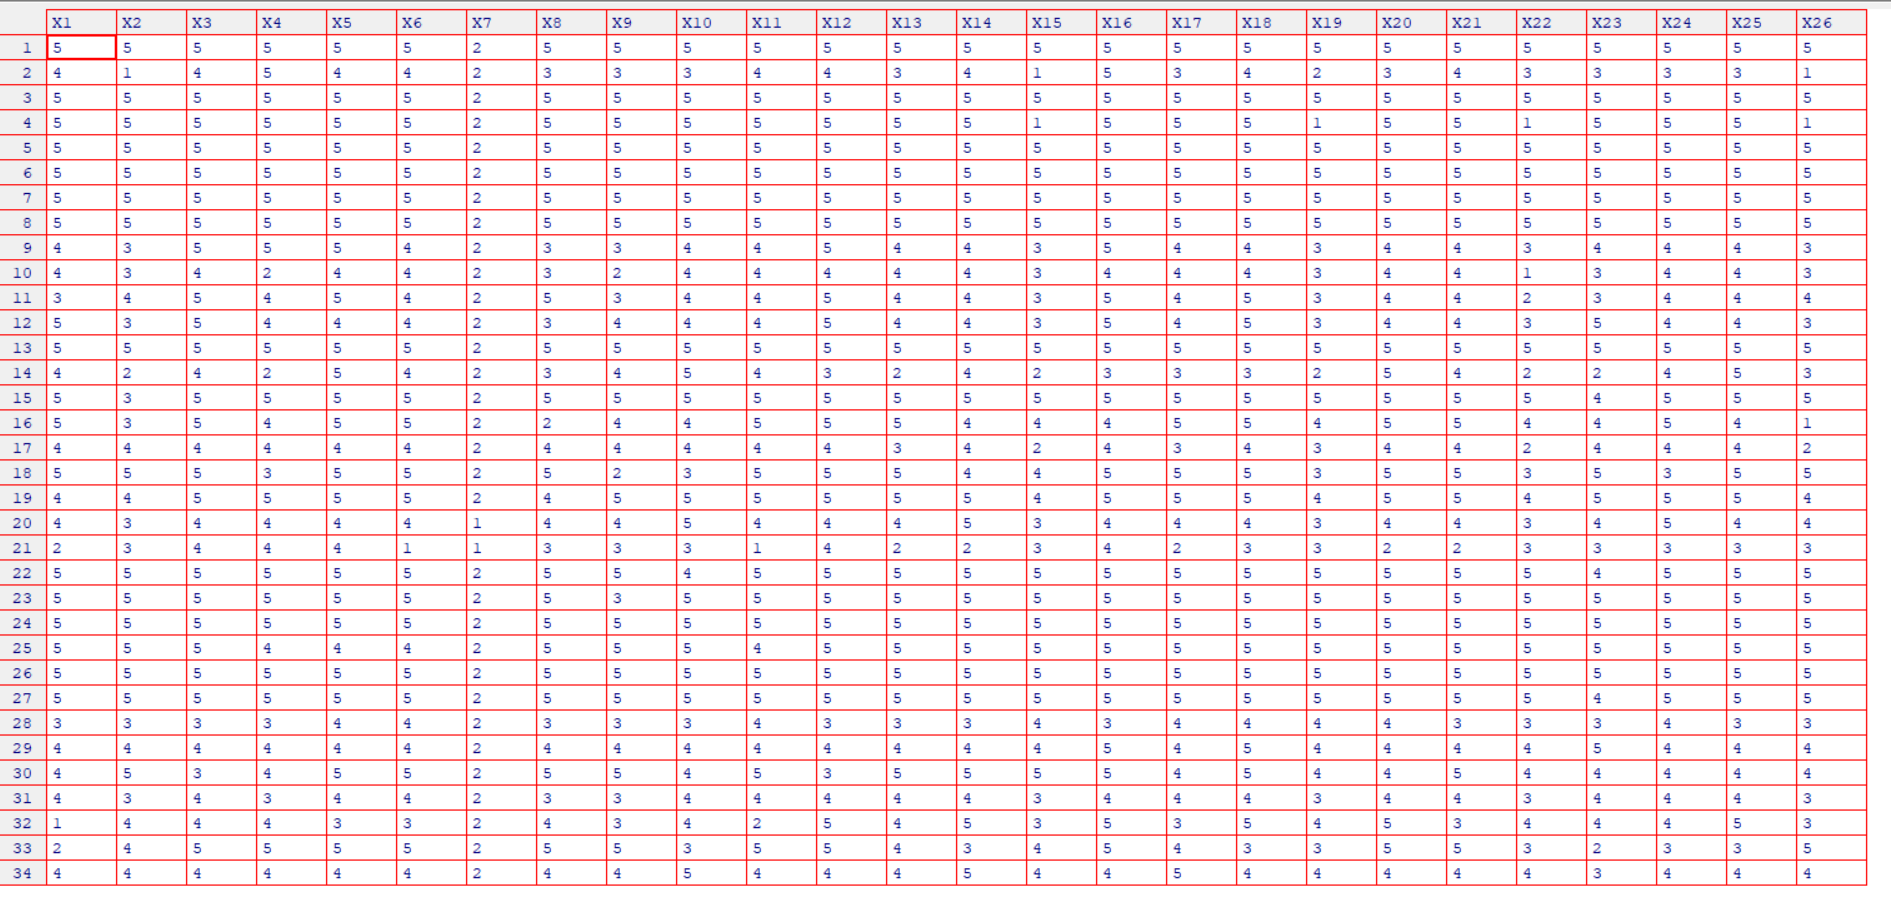
\includegraphics[width=\textwidth]{../../assets/images/data2b.png}
    \caption{Dữ liệu sau khi xáo trộn}
    \label{fig:shuffled_data}
\end{figure}

Để khám phá và xác định cấu trúc tiềm ẩn của dữ liệu, quy trình phân tích được triển khai theo hai bước:

\begin{enumerate}
    \item \textbf{Phân tích thành phần chính (Principal Component Analysis -- PCA)}:
    \begin{itemize}
        \item Xác định số lượng thành phần chính có khả năng giải thích phần lớn phương sai của dữ liệu.
        \item Đánh giá mức độ tương quan giữa các biến quan sát và loại bỏ các biến có tải số thấp hoặc không đạt yêu cầu.
        \item Sử dụng kết quả biểu đồ Scree Plot và giá trị Eigenvalue để đề xuất số nhân tố tiềm năng cho bước EFA.
    \end{itemize}

    \item \textbf{Phân tích nhân tố khám phá (Exploratory Factor Analysis -- EFA)}:
    \begin{itemize}
        \item Xác nhận và nhóm các biến quan sát thành các nhân tố đại diện.
        \item Kiểm định độ tin cậy và tính hội tụ của các thang đo.
        \item Loại bỏ các biến có hệ số tải nhân tố thấp hoặc tải chéo cao.
    \end{itemize}
\end{enumerate}

Cách tiếp cận này đảm bảo quá trình trích xuất nhân tố được thực hiện có cơ sở thống kê vững chắc, đồng thời tối ưu hóa khả năng giải thích và ứng dụng của mô hình nghiên cứu, phục vụ cho các bước phân tích suy luận và đề xuất giải pháp nâng cao chất lượng dịch vụ thông tin thư viện.

\subsection*{Bắt đầu quy trình phân tích:}
\textbf{1. Phân tích thành phần chính (PCA):} 

\text{Đọc dữ liệu vào R và xử lý dữ liệu ban đầu để tiến hành phân tích với code sau:}
\begin{lstlisting}[style=Rstyle, caption={Đọc dữ liệu vào để tiến hành phân tích dữ liệu}]
# INSTALL AND LOAD REQUIRED PACKAGES
# List of required packages with specific versions (if needed)
packages <- c("psych", "GPArotation", "ggplot2", "corrplot", "factoextra", 
             "nFactors", "dplyr", "knitr", "kableExtra", "rmarkdown")

# Install only missing packages
installed <- rownames(installed.packages())
to_install <- setdiff(packages, installed)
if(length(to_install) > 0) install.packages(to_install)

# Load libraries with error handling
suppressPackageStartupMessages({
  library(psych)        # For factor analysis and reliability tests
  library(GPArotation)  # For factor rotation methods
  library(ggplot2)      # For advanced visualizations
  library(corrplot)     # For correlation matrix visualization
  library(factoextra)   # For PCA visualization
  library(nFactors)     # For determining number of factors
  library(dplyr)        # For data manipulation
  library(knitr)        # For reporting
  library(kableExtra)   # For nice tables
})

# DATA IMPORT AND PREPROCESSING ================================================

# Read data from CSV file with error handling
tryCatch({
  setwd("D:/09_ThayLy/Chuyen_de_thong_ke_nang_cao/EFA")
  data <- read.csv("Data2b.csv", header = TRUE, stringsAsFactors = FALSE)
}, error = function(e) {
  stop("Error reading data file. Please check file path and format.")
})

# Initial data inspection
cat("\n=== DATA STRUCTURE ===\n")
str(data)
cat("\nFirst 5 rows:\n")
print(head(data, 5))

# Check for missing values
missing_values <- sum(is.na(data))
if(missing_values > 0) {
  cat("\nWarning:", missing_values, "missing values found.\n")
  # Visualize missing values
  if(require(visdat)) {
    visdat::vis_miss(data)
  }
} else {
  cat("\nNo missing values found.\n")
}

# Handle missing values by listwise deletion
data_clean <- na.omit(data)
cat("\nOriginal data:", nrow(data), "rows")
cat("\nAfter removing NAs:", nrow(data_clean), "rows")

# Check for zero variance variables
zero_var <- sapply(data_clean, function(x) var(x, na.rm = TRUE) == 0)
if(any(zero_var)) {
  cat("\nWarning: Zero variance variables detected:", names(data_clean)[zero_var], "\n")
  data_clean <- data_clean[, !zero_var]
}
\end{lstlisting}

\text{Sau đó, tiến hành kiểm định tương quan giữa các biến:}
\begin{lstlisting}[caption={Phân tích tương quan giữa các biến}]
# CORRELATION ANALYSIS ========================================================

# Calculate correlation matrix with handling for non-numeric columns
cor_matrix <- cor(data_clean[, sapply(data_clean, is.numeric)])

# Create publication-ready correlation plot
corr_plot <- function(cor_matrix) {
  corrplot(cor_matrix, 
           method = "color", 
           type = "upper",
           order = "hclust",
           tl.col = "black", 
           tl.srt = 45,
           tl.cex = 0.7,
           addCoef.col = "black",
           number.cex = 0.5,
           diag = FALSE,
           col = colorRampPalette(c("#BB4444", "#EE9988", "#FFFFFF", "#77AADD", "#4477AA"))(200),
           mar = c(0, 0, 1, 0))
 }

# Save correlation plot to file
png("correlation_matrix.png", width = 14, height = 12, units = "in", res = 300)
corr_plot(cor_matrix)
dev.off()
\end{lstlisting}

Kết quả kiểm định được minh họa bởi ma trận tương quan sau:
\begin{figure}[h!]
    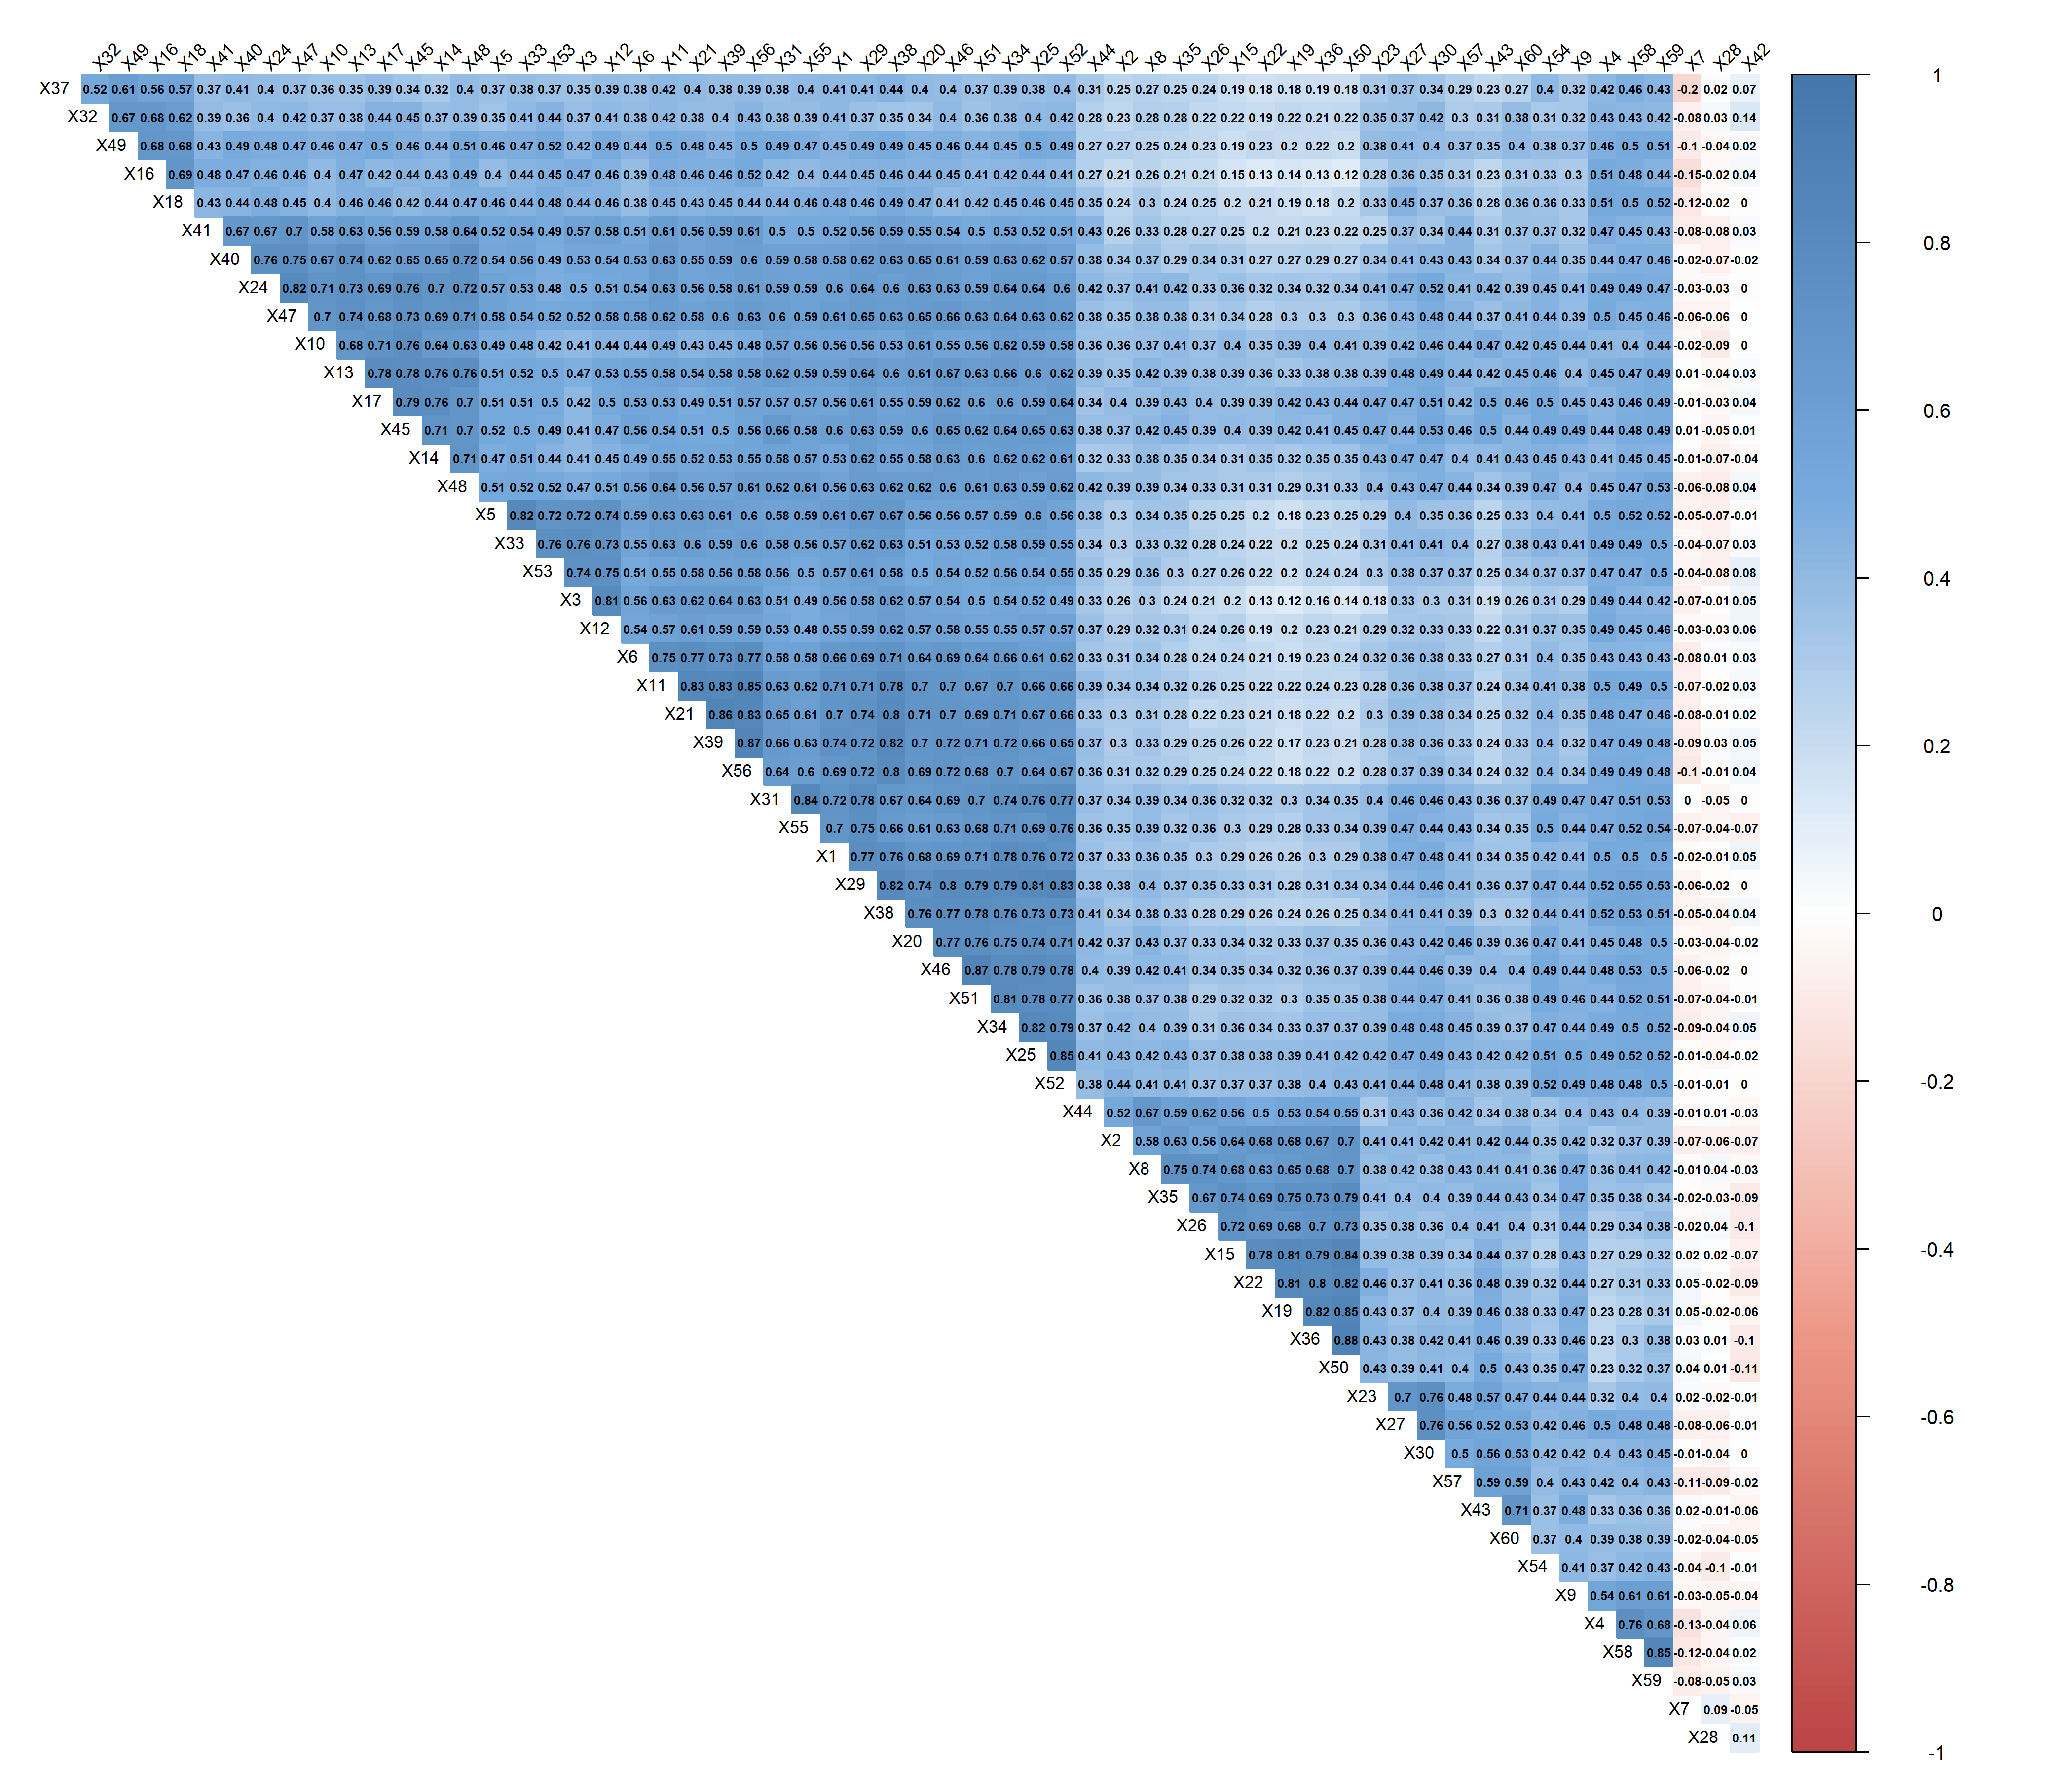
\includegraphics[width=\textwidth]{../../assets/images/correlation_matrix_1.png}
    \caption{Ma trận tương quan giữa các biến}
    \label{fig:correlation_matrix}
\end{figure}

\textbf{Đánh giá độ phù hợp của dữ liệu trước khi phân tích:}
\begin{itemize}
    \item Kiểm định Kaiser-Meyer-Olkin (KMO):
    \begin{lstlisting}
# ASSUMPTION CHECKS FOR FACTOR ANALYSIS =======================================

# Kaiser-Meyer-Olkin (KMO) Measure of Sampling Adequacy
kmo_check <- function(data) {
  kmo_result <- KMO(data)
  cat("\n=== KMO TEST RESULTS ===\n")
  print(kmo_result)
  
  # Interpretation
  kmo_overall <- kmo_result$MSA
  cat("\nKMO Overall:", kmo_overall, "\n")
  if(kmo_overall >= 0.90) {
    cat("Interpretation: Marvelous\n")
  } else if(kmo_overall >= 0.80) {
    cat("Interpretation: Meritorious\n")
  } else if(kmo_overall >= 0.70) {
    cat("Interpretation: Middling\n")
  } else if(kmo_overall >= 0.60) {
    cat("Interpretation: Mediocre\n")
  } else {
    cat("Interpretation: Unacceptable\n")
  }
  
  # Identify problematic variables (MSA < 0.5)
  bad_vars <- names(which(kmo_result$MSAi < 0.5))
  if(length(bad_vars) > 0) {
    cat("\nVariables with KMO < 0.5 (consider removing):\n")
    print(bad_vars)
  }
  
  return(kmo_result)
}

kmo_result <- kmo_check(data_clean)
    \end{lstlisting}
    
    Kết quả cho thấy KMO = 0.97, đạt mức "Marvelous" cho thấy dữ liệu rất phù hợp để tiến hành phân tích nhân tố.

\item Kiểm định Bartlett's Test
    \begin{lstlisting}[caption={Code kiểm định Bartlett's Test}]
# Bartlett's Test of Sphericity
bartlett_check <- function(data) {
  result <- cortest.bartlett(data)
  
  cat("\n=== BARTLETT'S TEST ===\n")
  cat("Chi-square:", round(result$chisq, 2), "\n")
  cat("p-value:", ifelse(result$p.value < 0.001, "< 0.001", round(result$p.value, 4)), "\n")
  
  if(result$p.value < 0.05) {
    cat("Result: Significant (data suitable for factor analysis)\n")
  } else {
    cat("Result: Not significant (data may not be suitable)\n")
  }
  
  return(result)
}

bartlett_result <- bartlett_check(data_clean)
    \end{lstlisting}
\end{itemize}

Tiến hành kiểm định PCA, với chương trình code như sau:
\begin{lstlisting}
# PRINCIPAL COMPONENT ANALYSIS (PCA) ==========================================

# Enhanced PCA function with automatic reporting
run_pca <- function(data, scale = TRUE) {
  pca_result <- prcomp(data, scale. = scale)
  
  # Variance explained
  variance <- pca_result$sdev^2
  prop_var <- variance / sum(variance)
  cum_var <- cumsum(prop_var)
  
  # Create summary table
  pca_summary <- data.frame(
    Component = 1:length(pca_result$sdev),
    Eigenvalue = variance,
    Proportion = prop_var,
    Cumulative = cum_var
  )
  
  cat("\n=== PCA SUMMARY ===\n")
  print(pca_summary)
  
  # Determine number of components
  n_components <- sum(variance > 1) # Kaiser's rule
  cat("\nNumber of components with eigenvalue > 1:", n_components, "\n")
  
  return(list(
    pca = pca_result,
    summary = pca_summary,
    n_components = n_components
  ))
}

pca_results <- run_pca(data_clean)
\end{lstlisting}

Kết quả cho thấy 10 thành phần chính đầu tiên giải thích được 75.80\% tổng phương sai, với thành phần đầu tiên giải thích 45.70\% phương sai.

\begin{figure}[h!]
    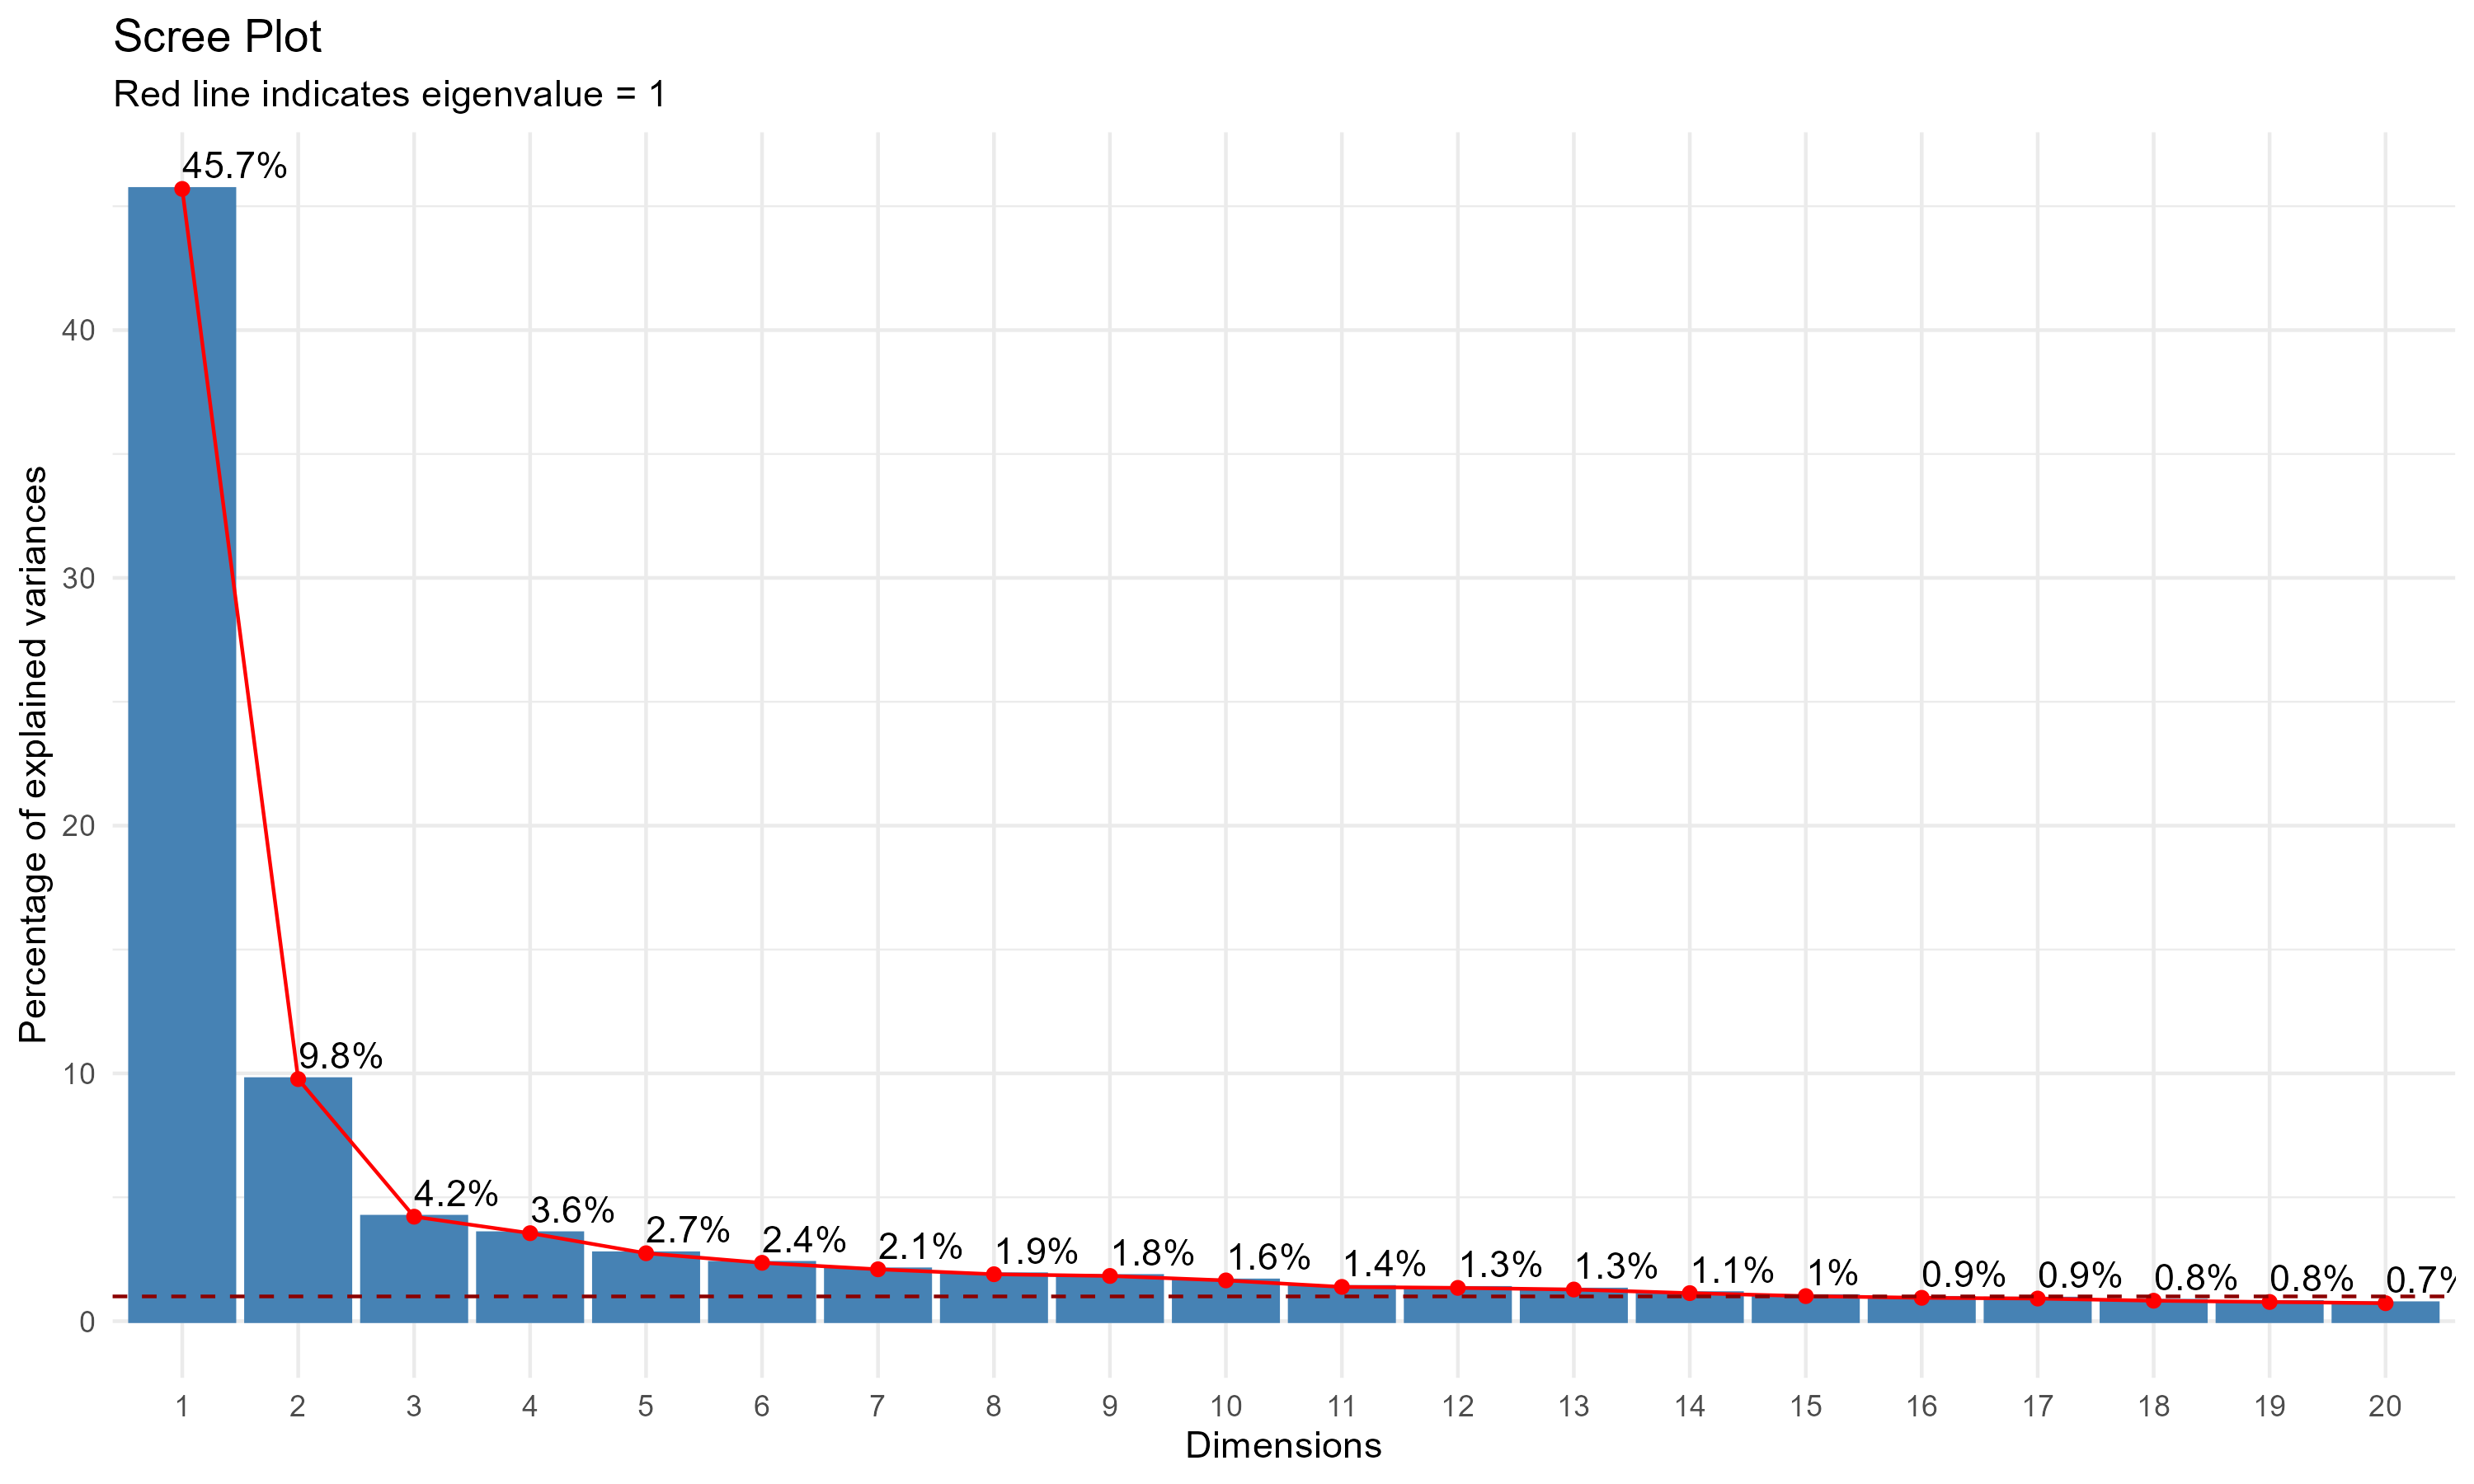
\includegraphics[width=\textwidth]{../../assets/images/SP42.png}
    \caption{Minh họa thành phần phương sai đóng góp}
    \label{fig:scree_plot}
\end{figure}

\begin{figure}[h!]
    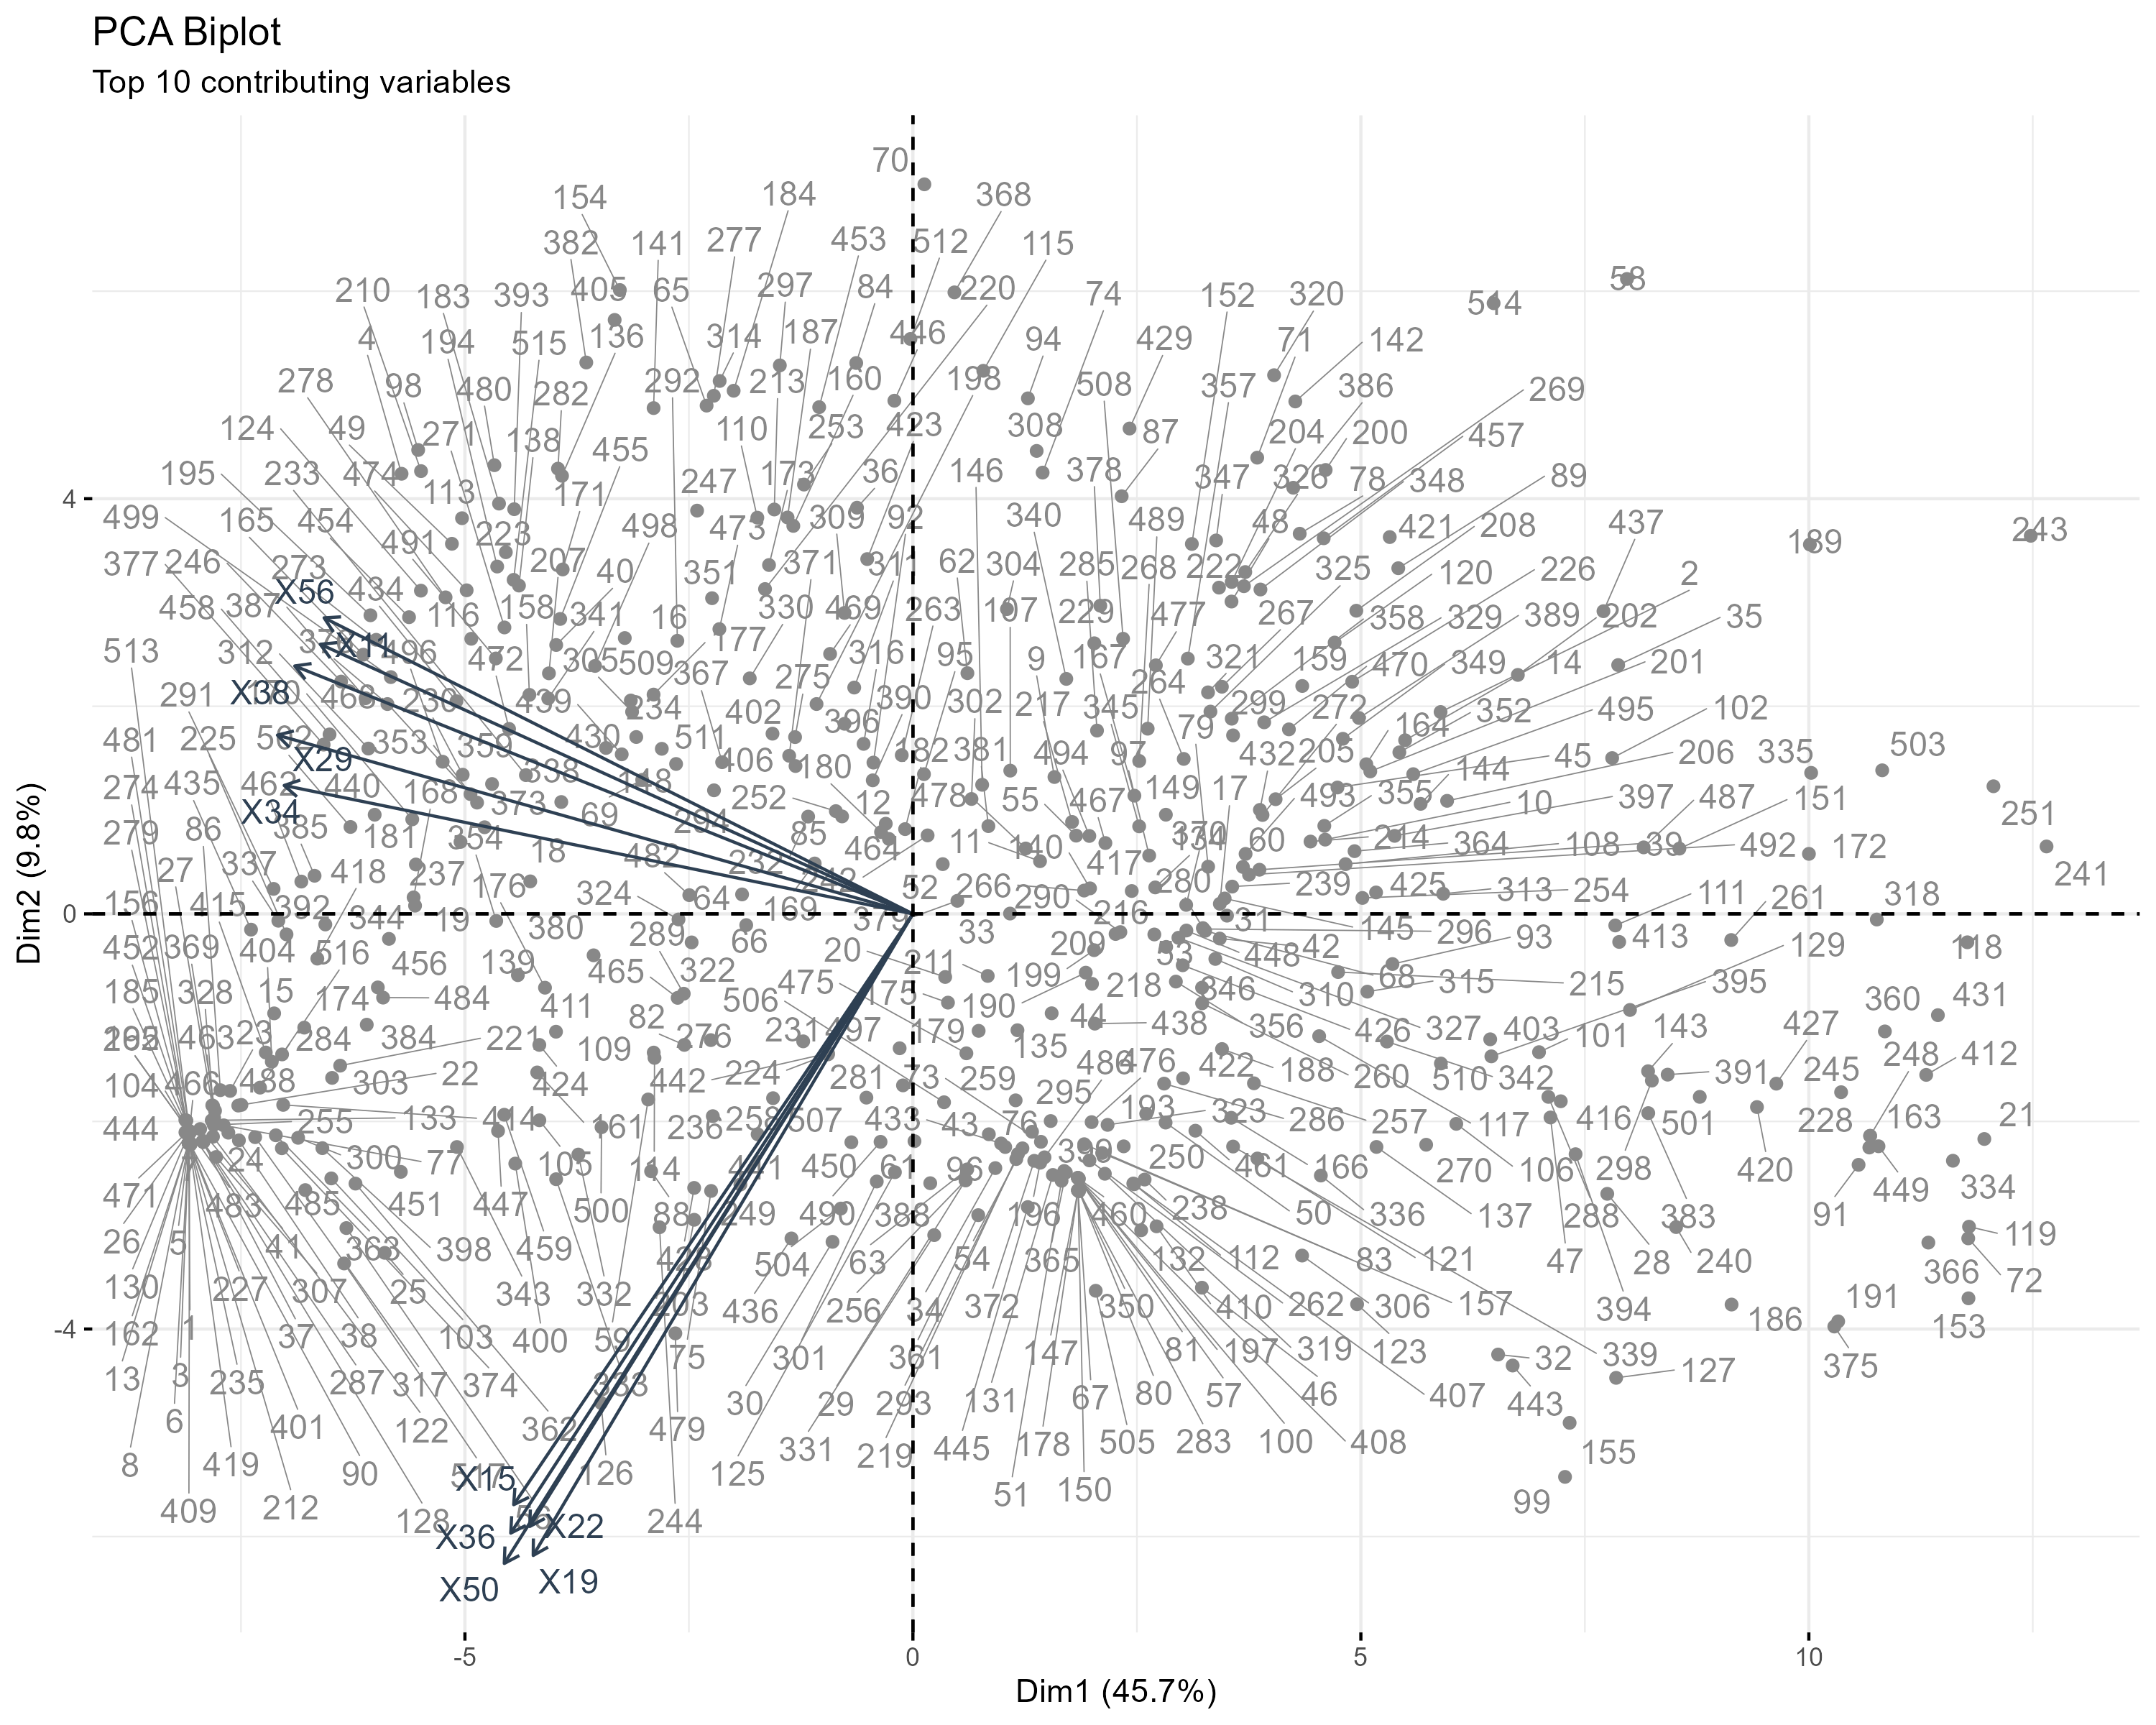
\includegraphics[width=0.9\textwidth]{../../assets/images/SP43.png}
    \caption{Top 10 các biến đóng góp}
    \label{fig:contributions}
\end{figure}

\subsection{Bước 5: Phân tích nhân tố khám phá (EFA)}

Với dữ liệu trên, tiếp tục phân tích nhân tố khám phá (EFA) với chương trinh R như sau:

\begin{lstlisting}
# EXPLORATORY FACTOR ANALYSIS (EFA) ===========================================

# Enhanced EFA function with rotation options and diagnostics
run_efa <- function(data, nfactors = NULL, rotate = "varimax", fm = "ml") {
  
  # Determine number of factors if not specified
  if(is.null(nfactors)) {
    cat("\nDetermining optimal number of factors...\n")
    parallel <- fa.parallel(data, 
                          fa = "fa",
                          n.iter = 100,
                          plot = FALSE)
    nfactors <- parallel$nfact
    cat("Suggested number of factors:", nfactors, "\n")
  }
  
  # Run EFA
  efa_result <- fa(data, 
                  nfactors = nfactors,
                  rotate = rotate,
                  fm = fm,
                  scores = "regression")
  
  # Print loadings with nice formatting
  cat("\n=== FACTOR LOADINGS ===\n")
  print(efa_result$loadings, cutoff = 0.4, sort = TRUE)
  
  return(list(
    efa = efa_result,
    nfactors = nfactors
  ))
}

# Run EFA analysis
efa_results <- run_efa(data_clean)
\end{lstlisting}

Kết quả phân tích EFA cho thấy 8 nhân tố được trích xuất, giải thích được 68.2\% tổng phương sai:

\begin{figure}[h!]
    \centering
        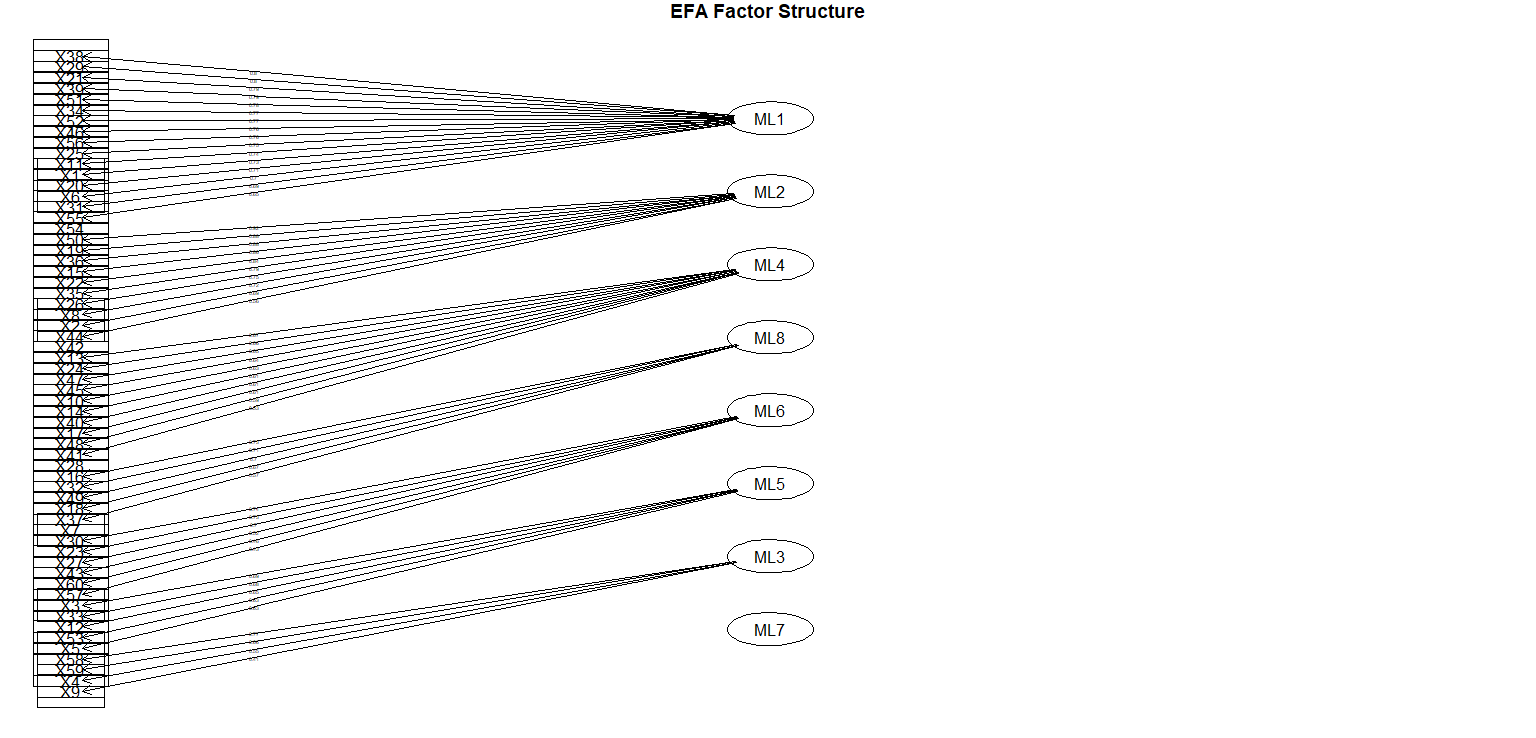
\includegraphics[width=1.5\linewidth]{../../assets/images/EFA_ML.png}
        \caption{Biểu đồ EFA tổng quát}
        \label{fig:efa_general}
\end{figure}

\subsection{Bước 6: Đánh giá độ tin cậy Cronbach's Alpha}

Đánh giá độ tin cậy cho từng nhân tố được trích xuất từ EFA:

\begin{figure}[h!]
    \centering
        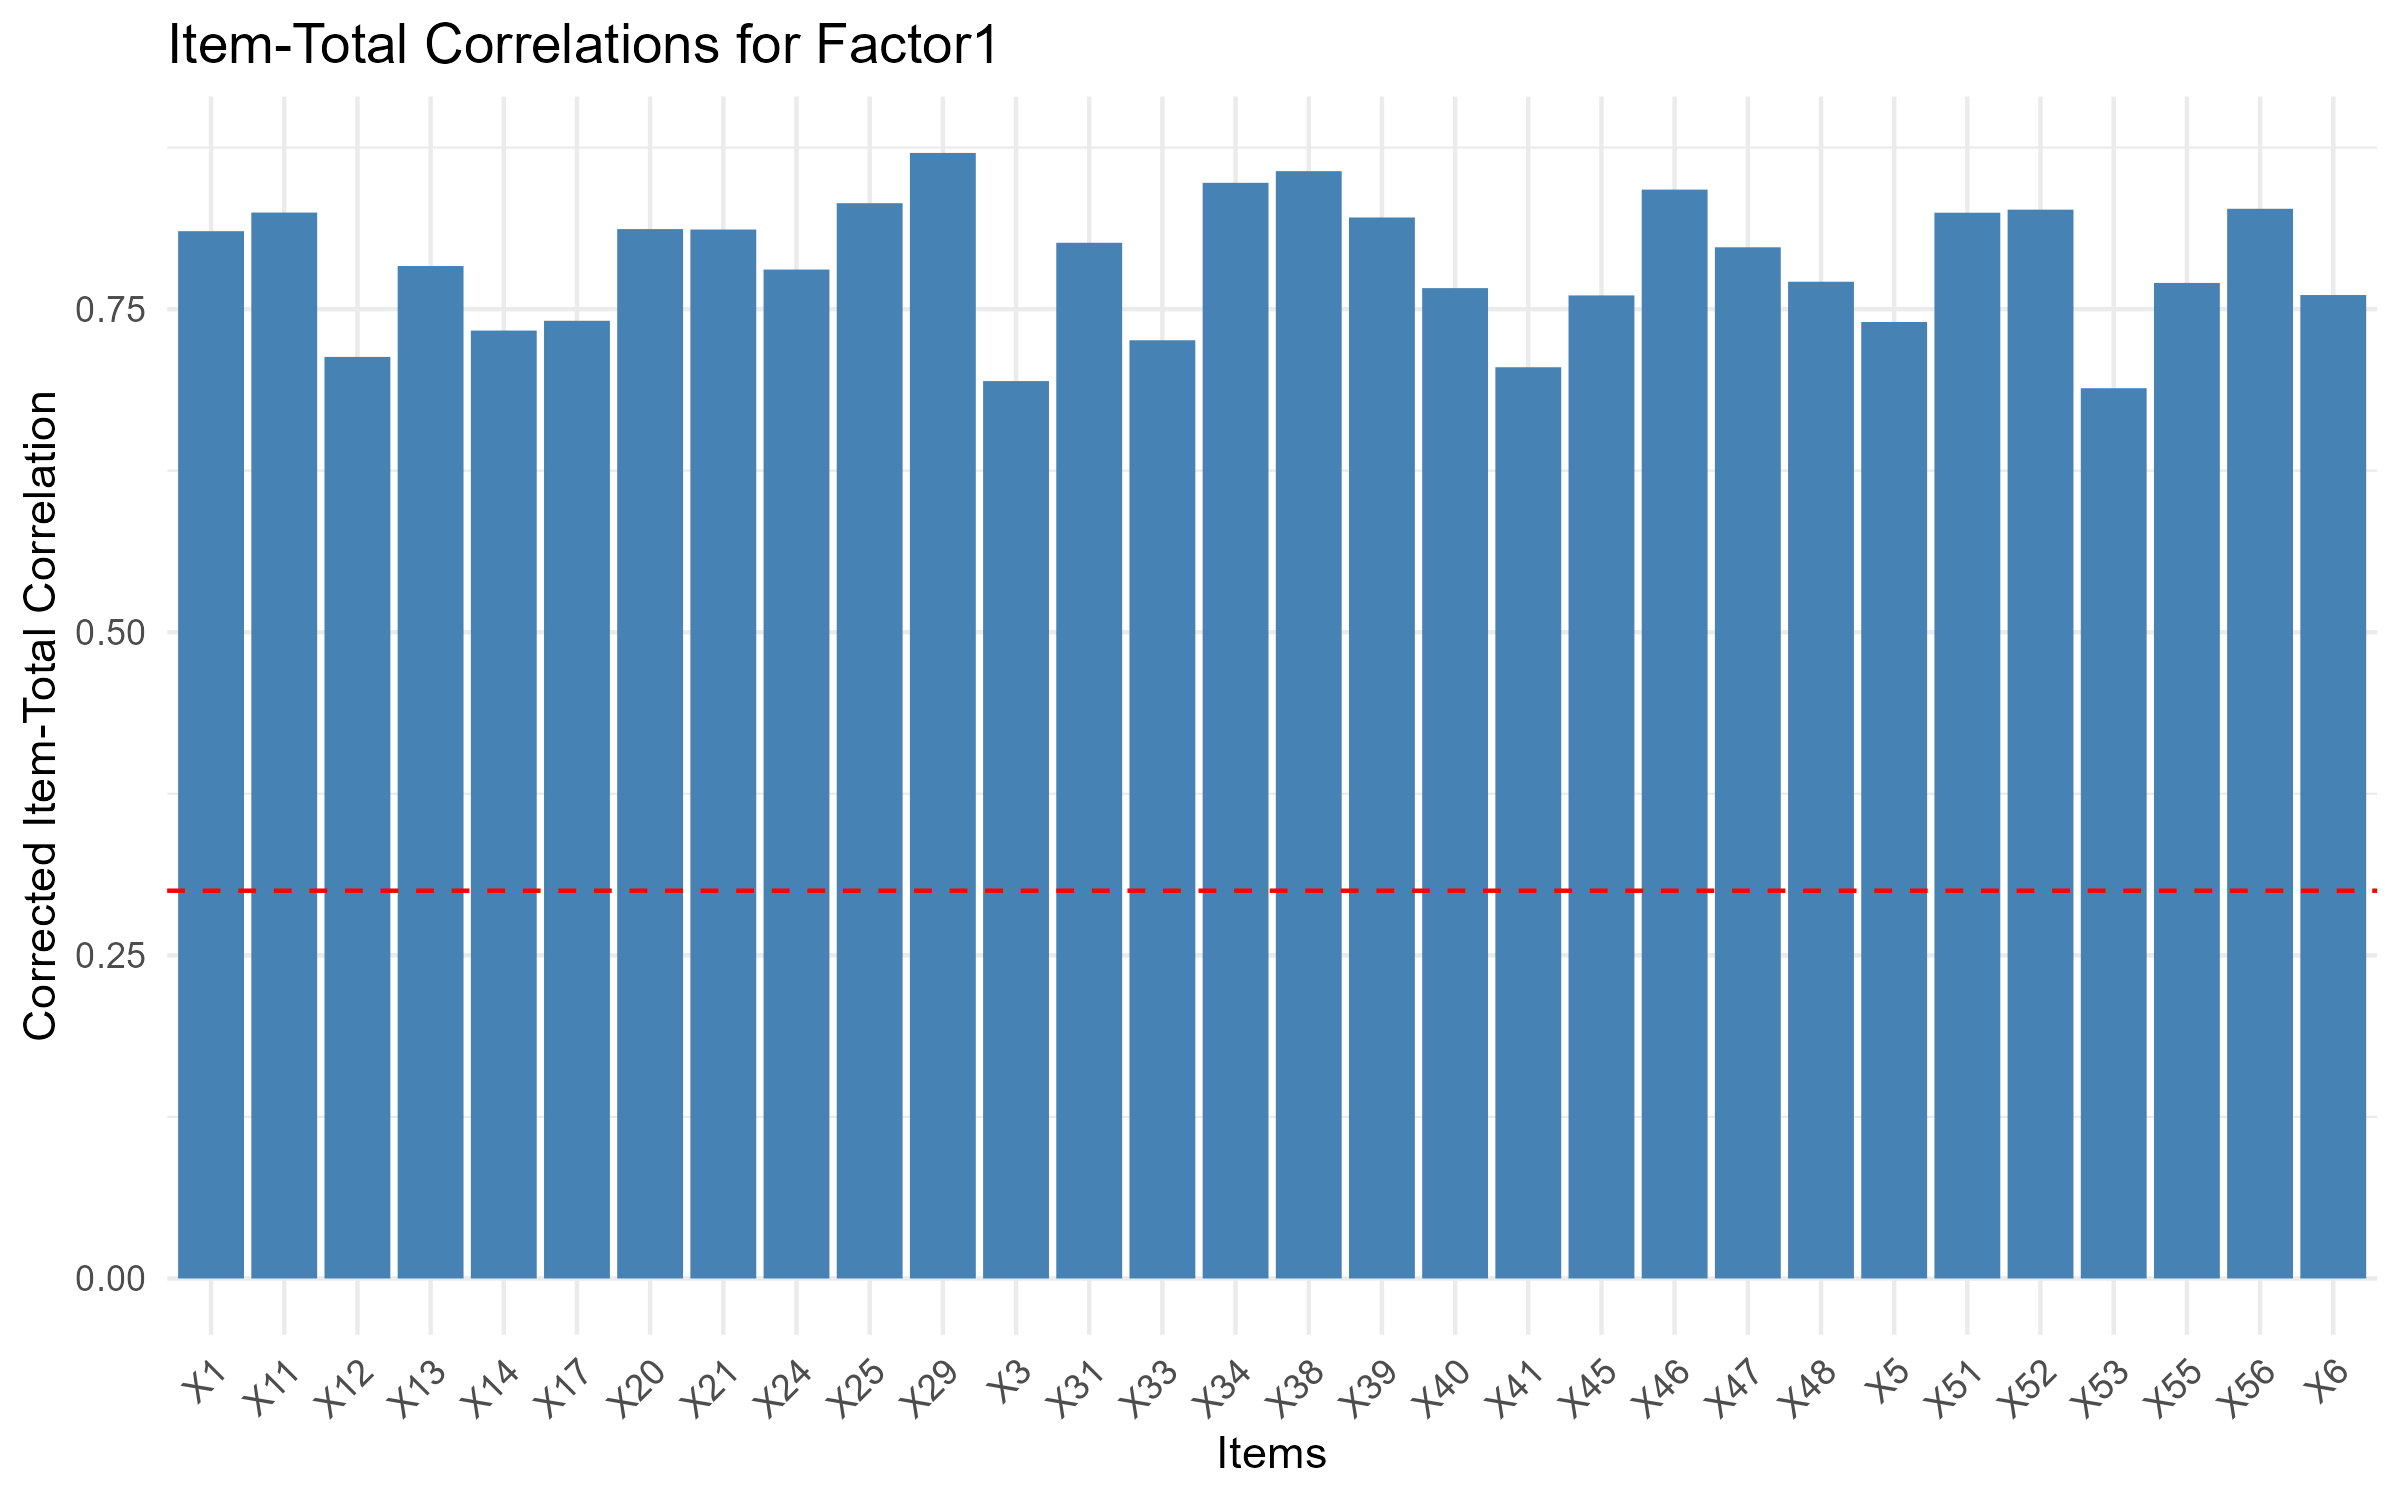
\includegraphics[width=0.55\linewidth]{../../assets/images/reliability_Factor1.png}
        \caption{Độ tin cậy Factor 1}
        \label{fig:reliability_f1}
\end{figure}

\begin{figure}[h!]
    \centering
    % Hàng 1 của 6 hình còn lại
    \begin{subfigure}[b]{0.45\linewidth}
        \centering
        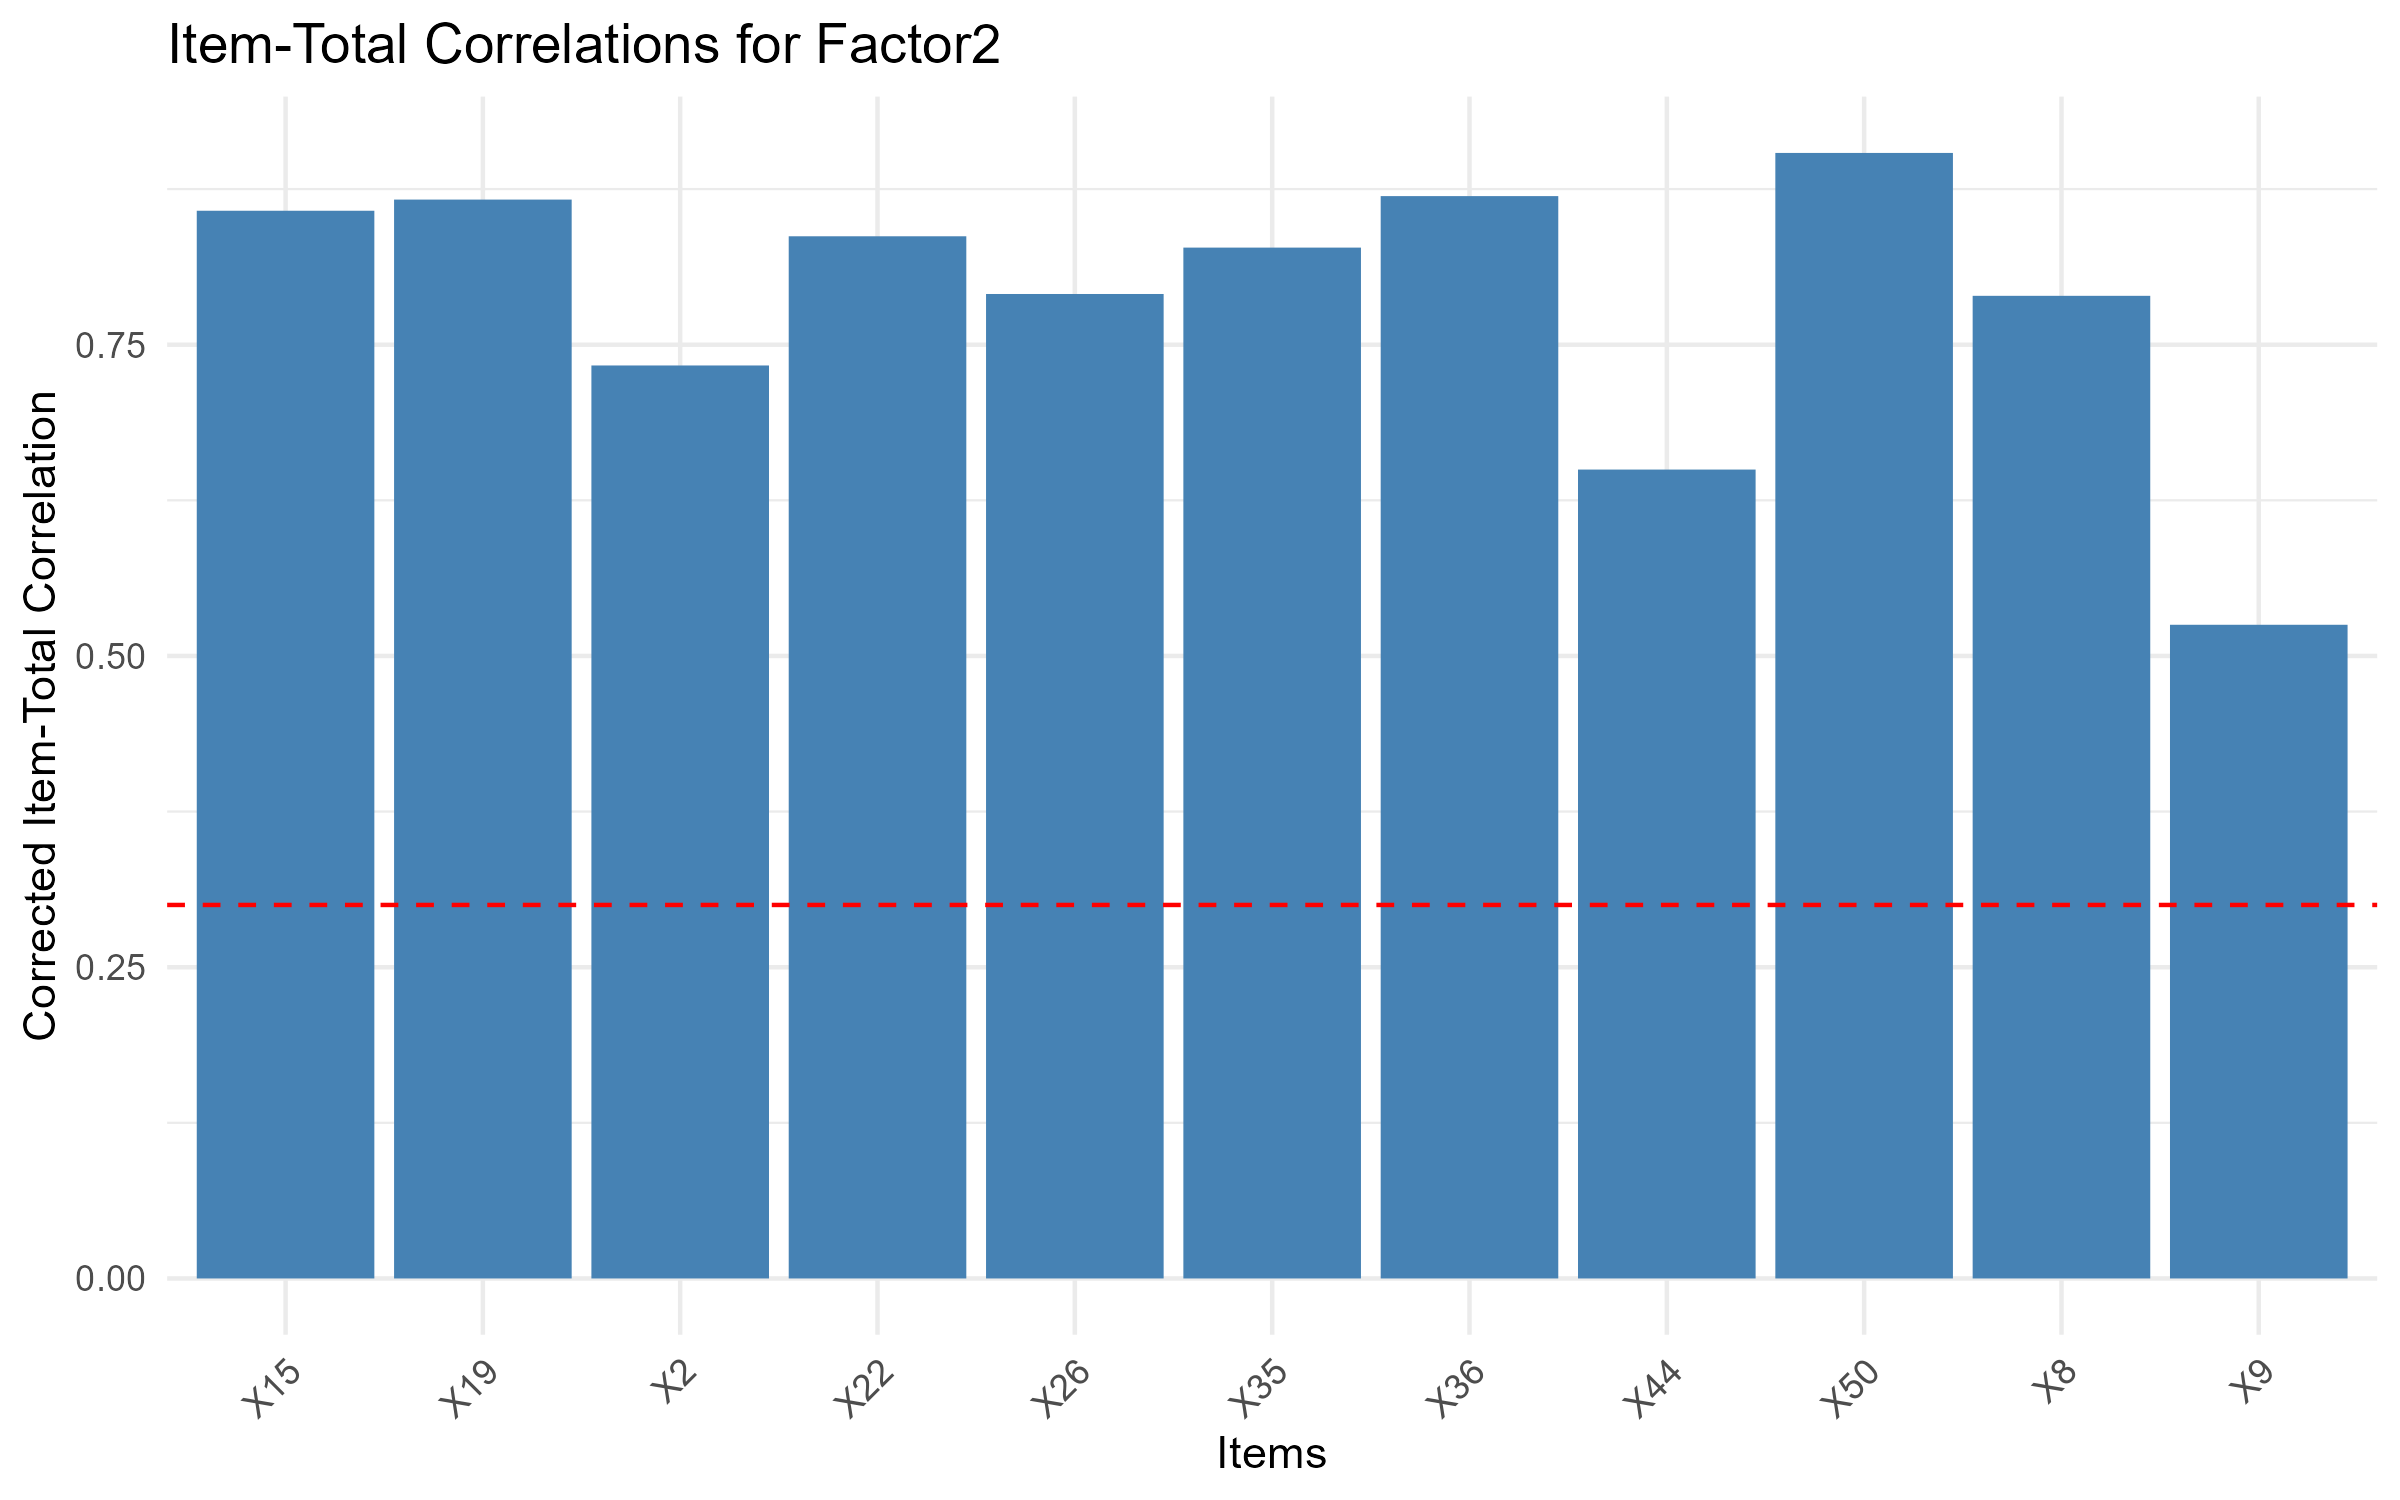
\includegraphics[width=\linewidth]{../../assets/images/reliability_Factor2.png}
        \caption{Độ tin cậy Factor 2}
        \label{fig:reliability_f2}
    \end{subfigure}
    \hfill
    \begin{subfigure}[b]{0.45\linewidth}
        \centering
        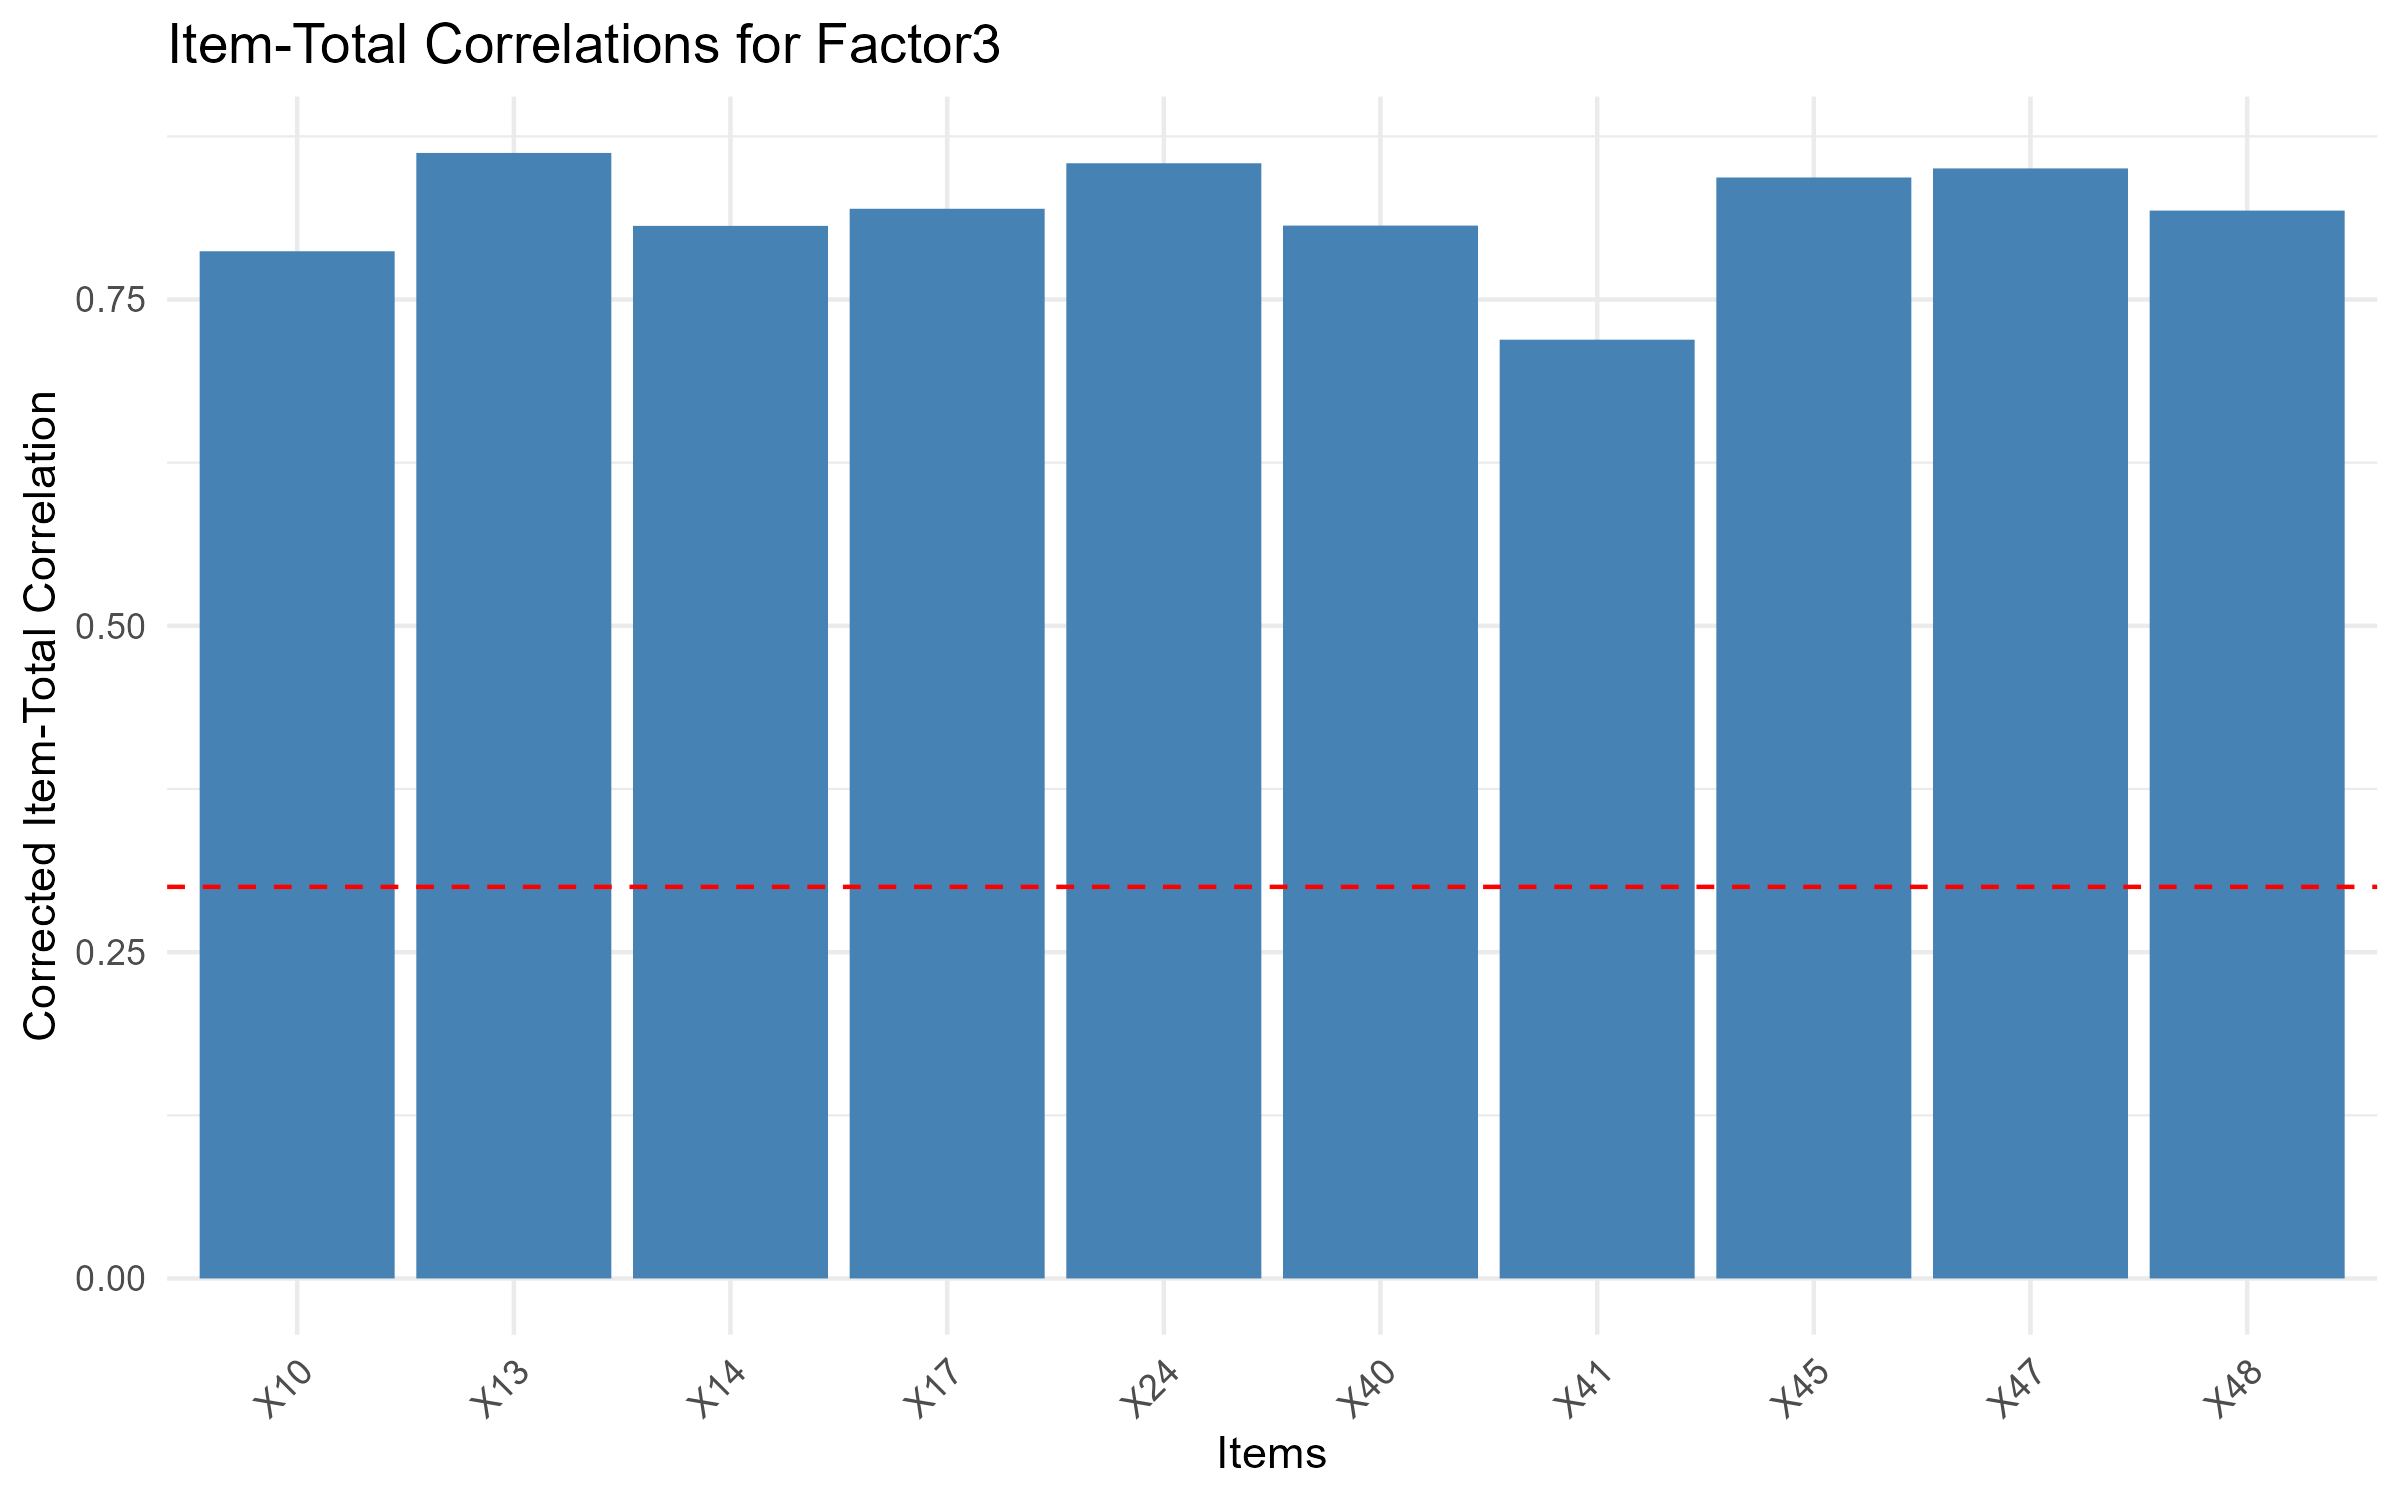
\includegraphics[width=\linewidth]{../../assets/images/reliability_Factor3.png}
        \caption{Độ tin cậy Factor 3}
        \label{fig:reliability_f3}
    \end{subfigure}

    \vskip 0.5cm
    % Hàng 2 của 6 hình còn lại
    \begin{subfigure}[b]{0.45\linewidth}
        \centering
        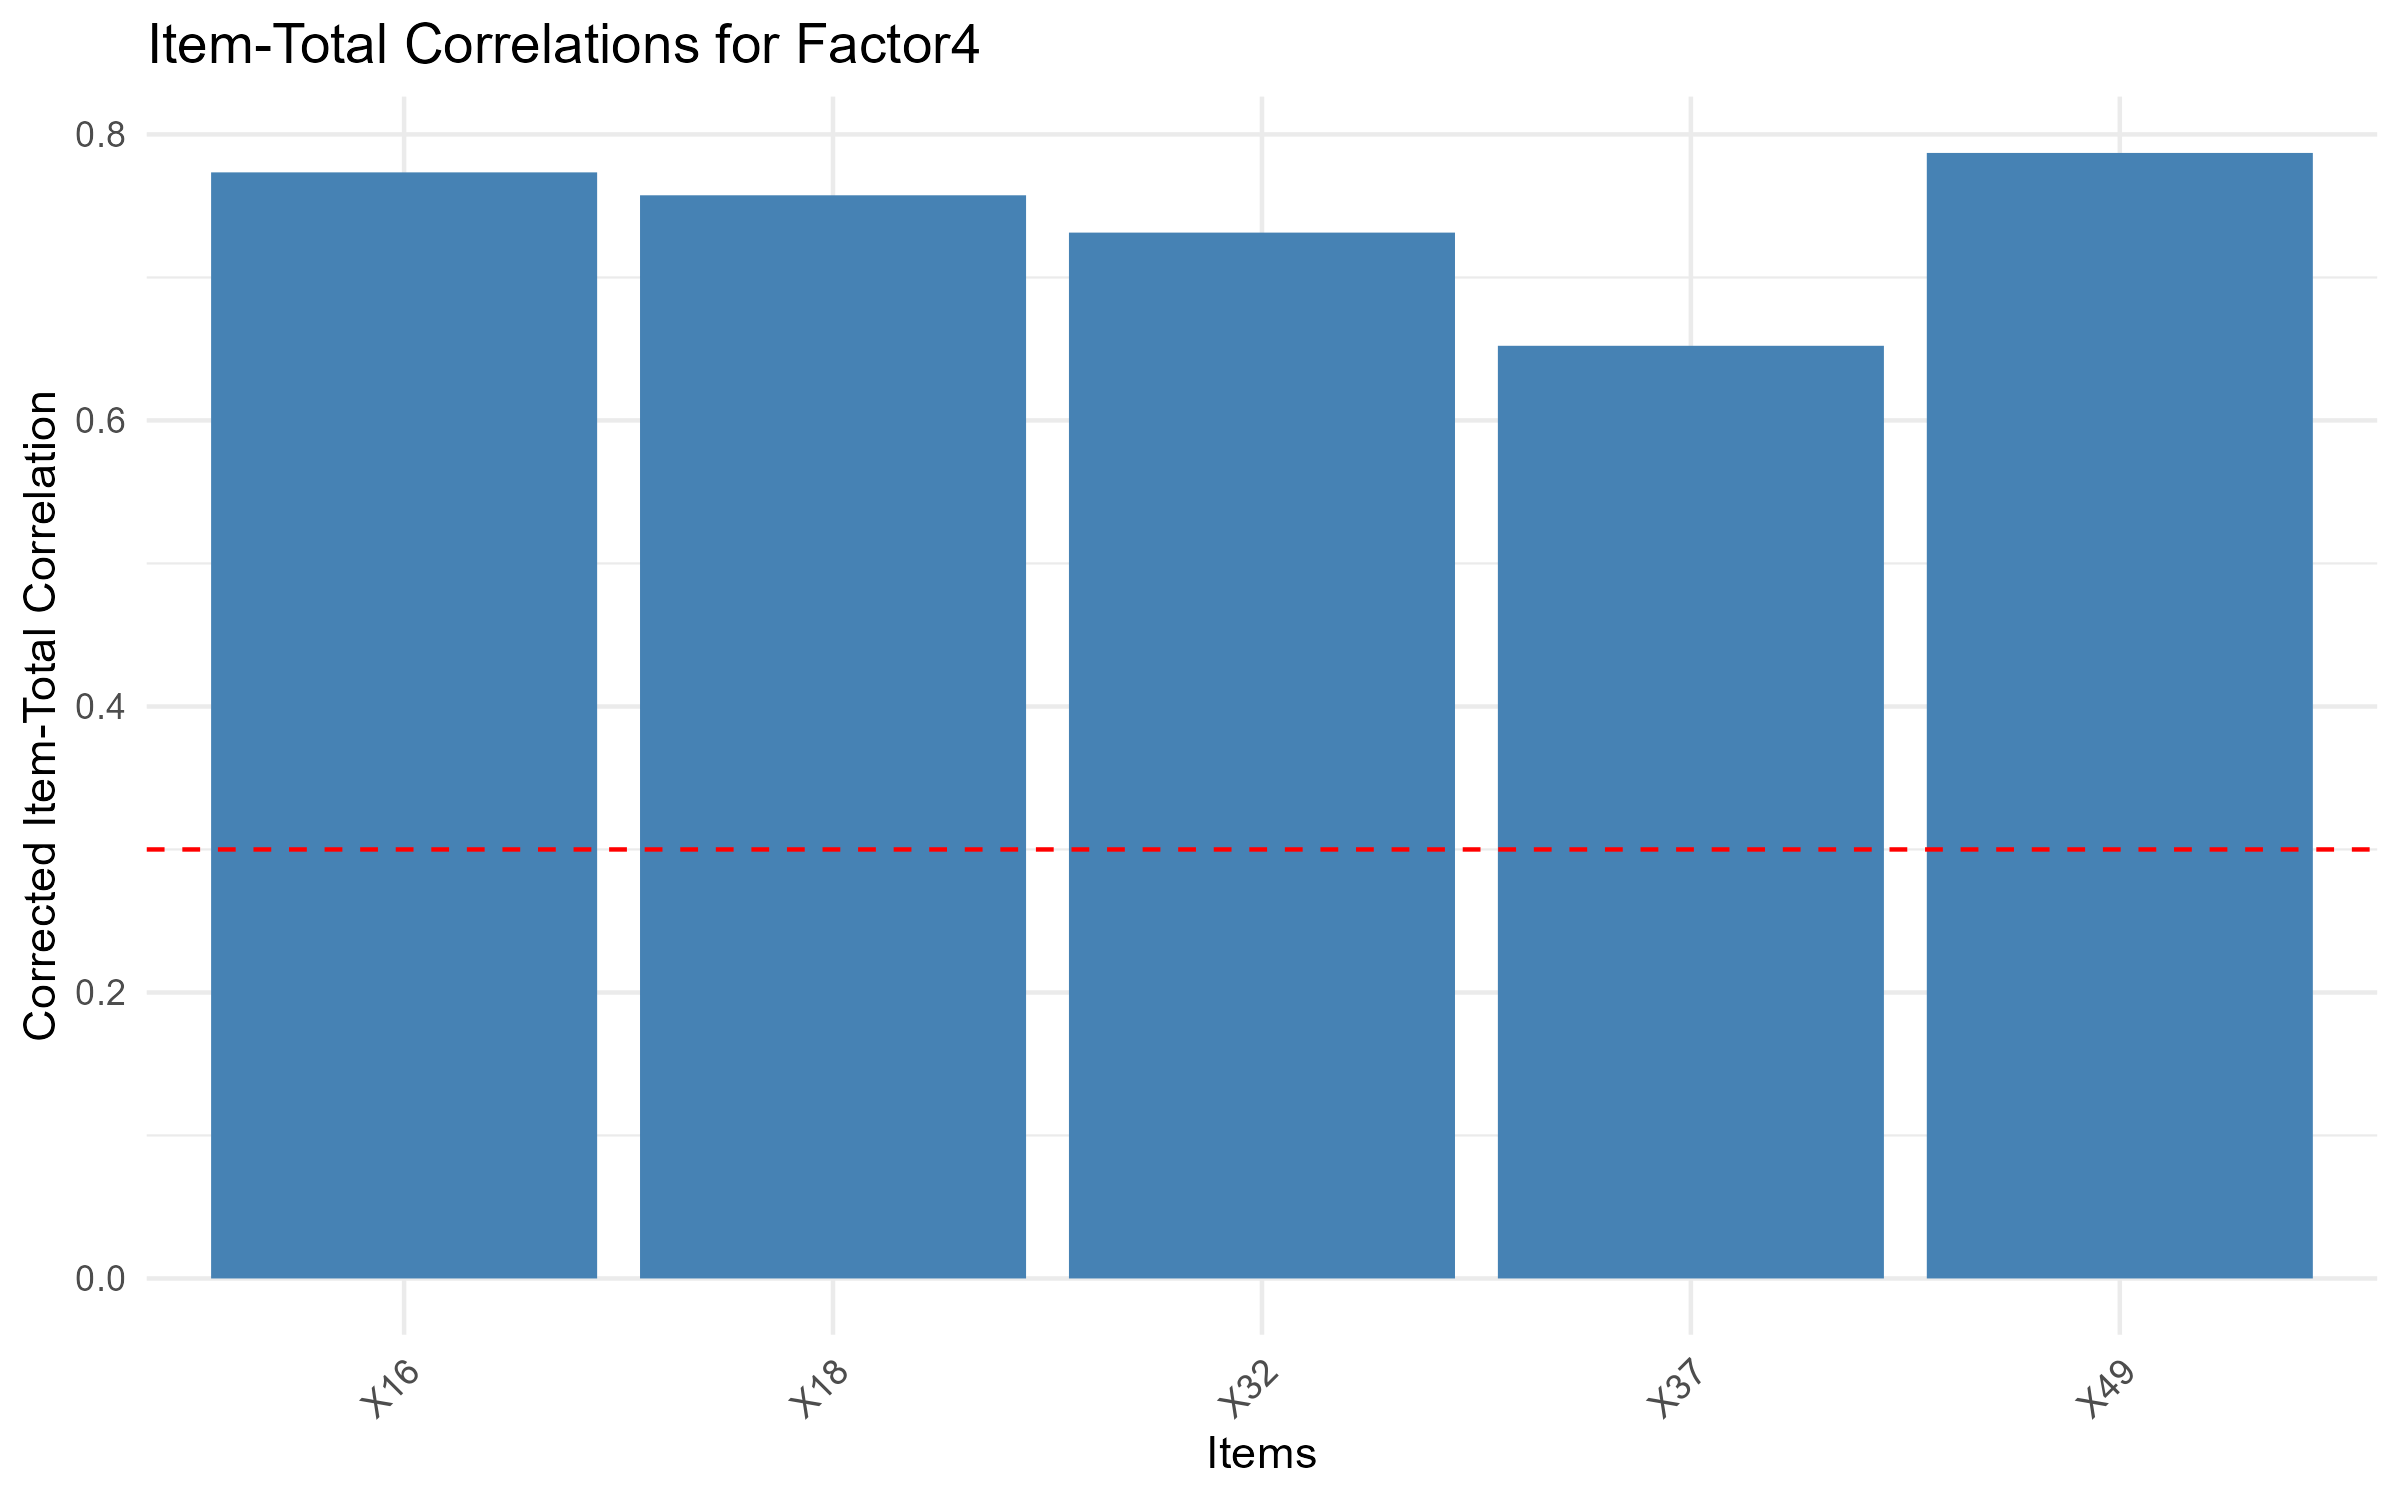
\includegraphics[width=\linewidth]{../../assets/images/reliability_Factor4.png}
        \caption{Độ tin cậy Factor 4}
        \label{fig:reliability_f4}
    \end{subfigure}
    \hfill
    \begin{subfigure}[b]{0.45\linewidth}
        \centering
        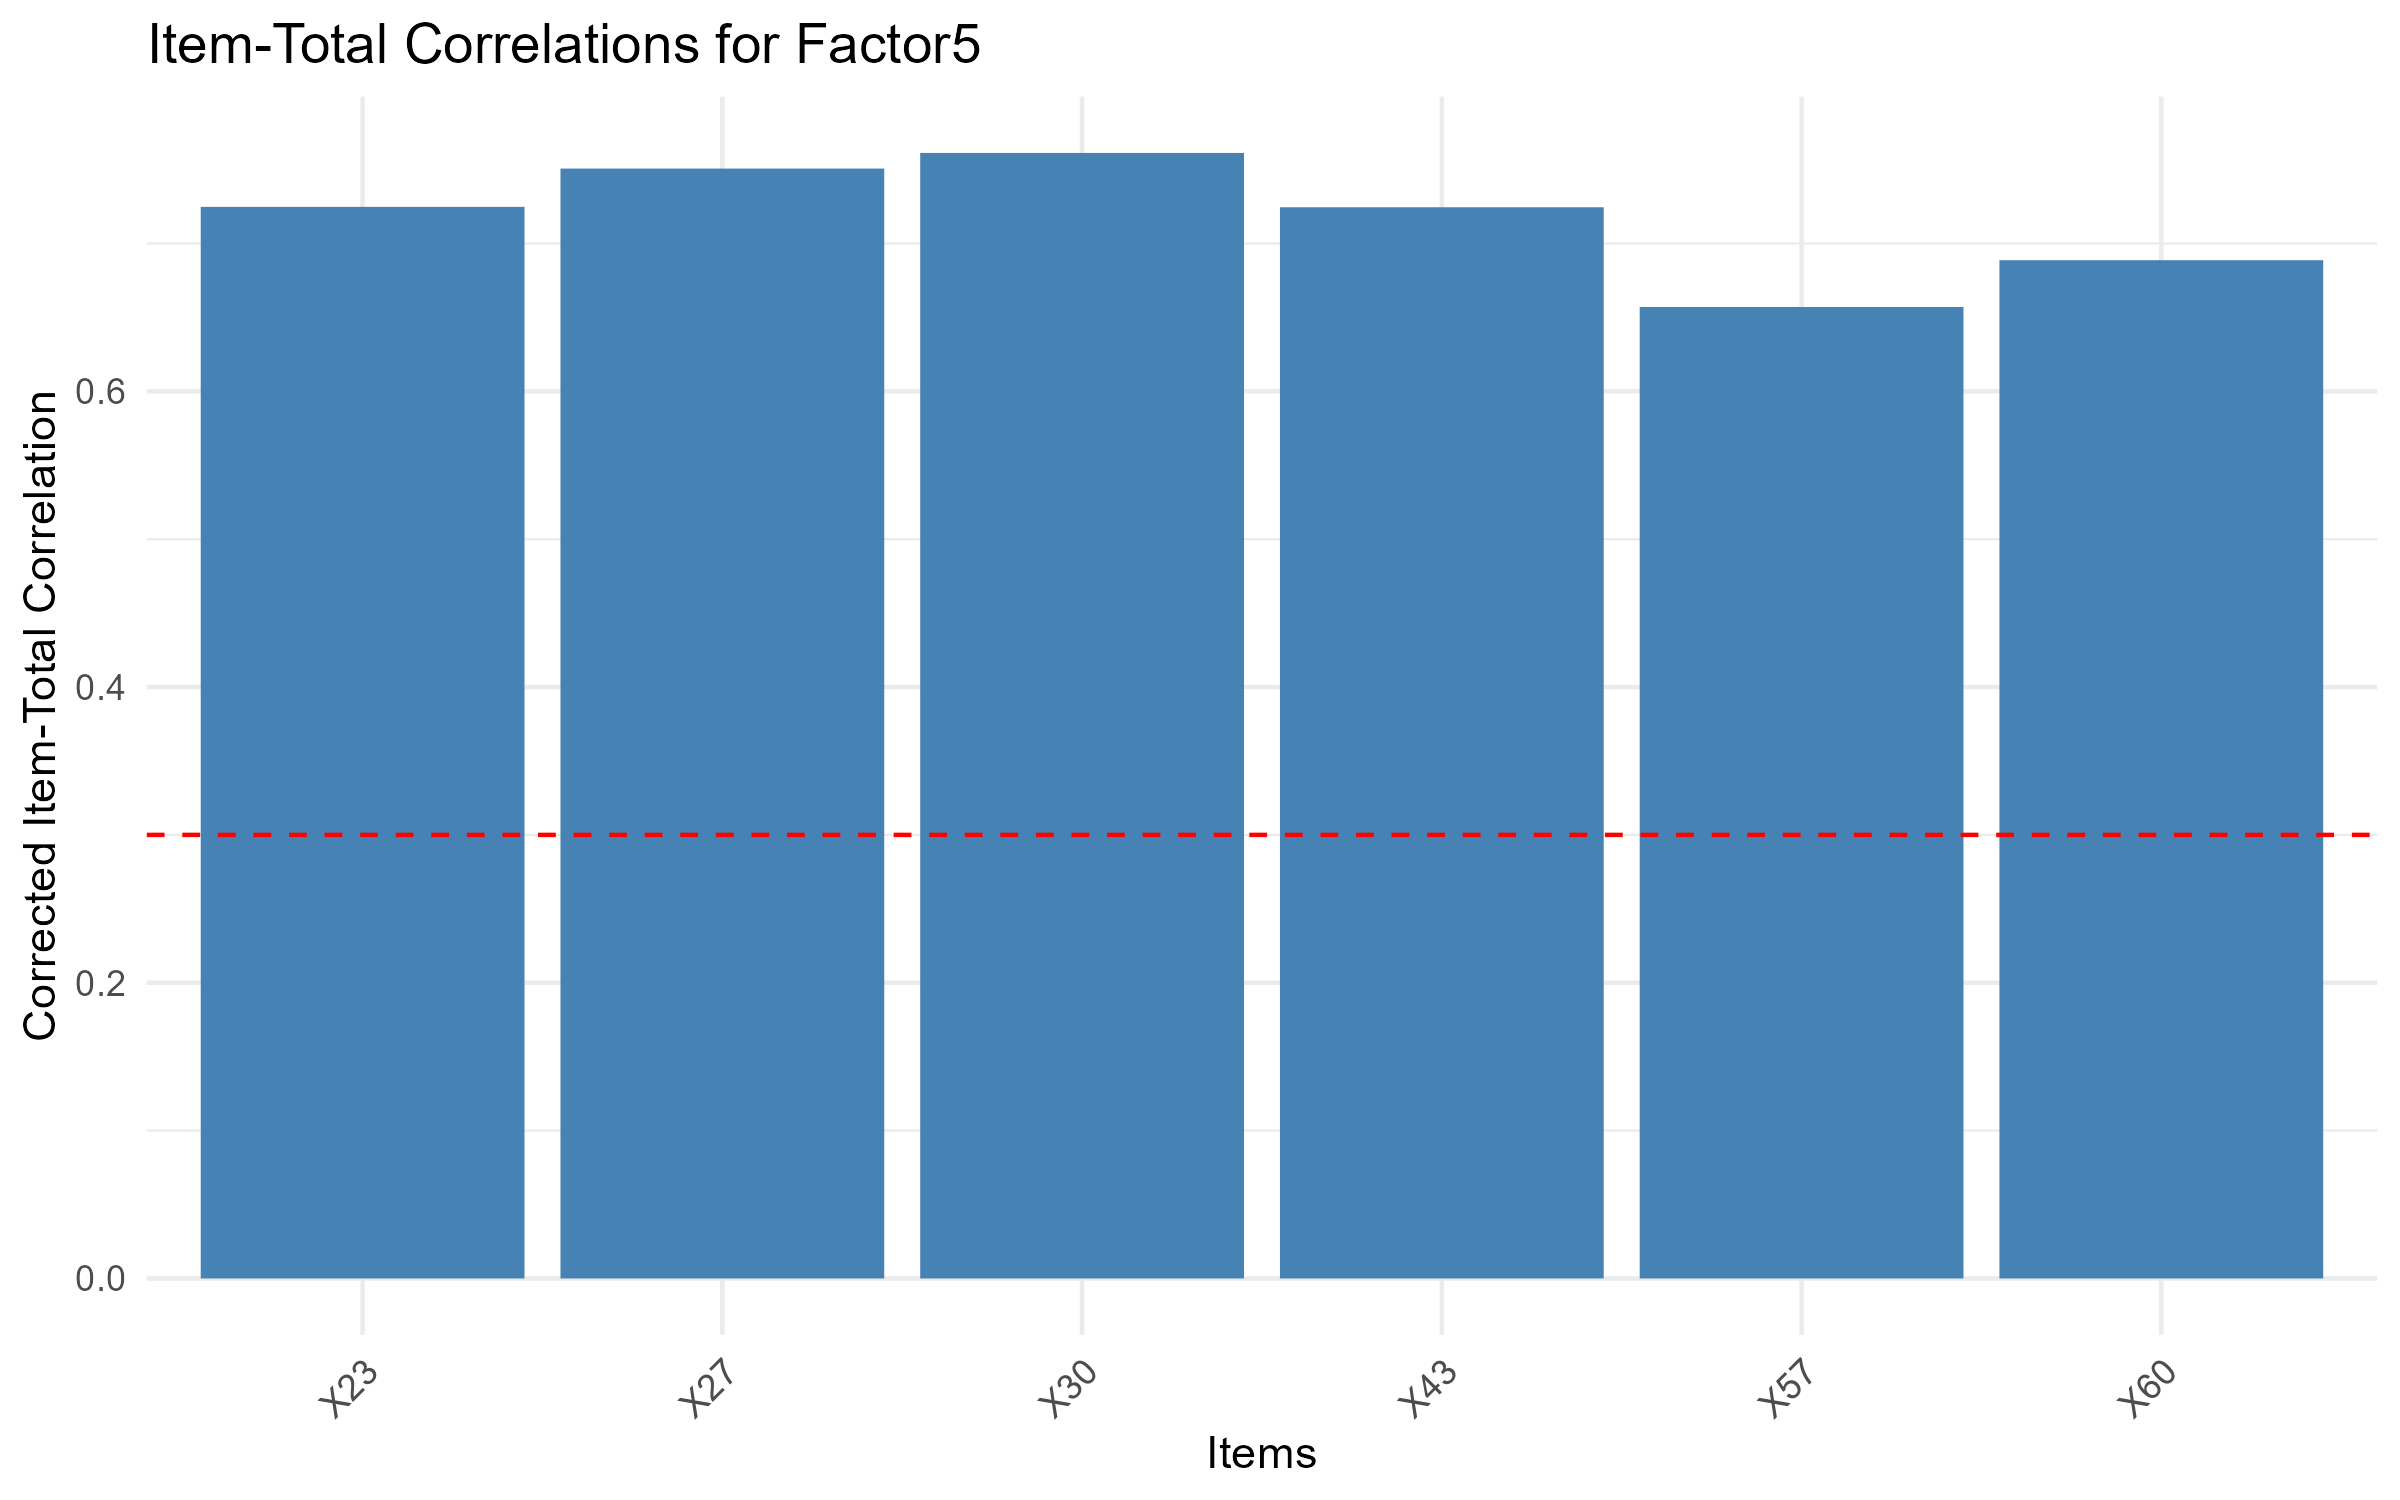
\includegraphics[width=\linewidth]{../../assets/images/reliability_Factor5.png}
        \caption{Độ tin cậy Factor 5}
        \label{fig:reliability_f5}
    \end{subfigure}

    \vskip 0.5cm
    % Hàng 3 của 6 hình còn lại
    \begin{subfigure}[b]{0.45\linewidth}
        \centering
        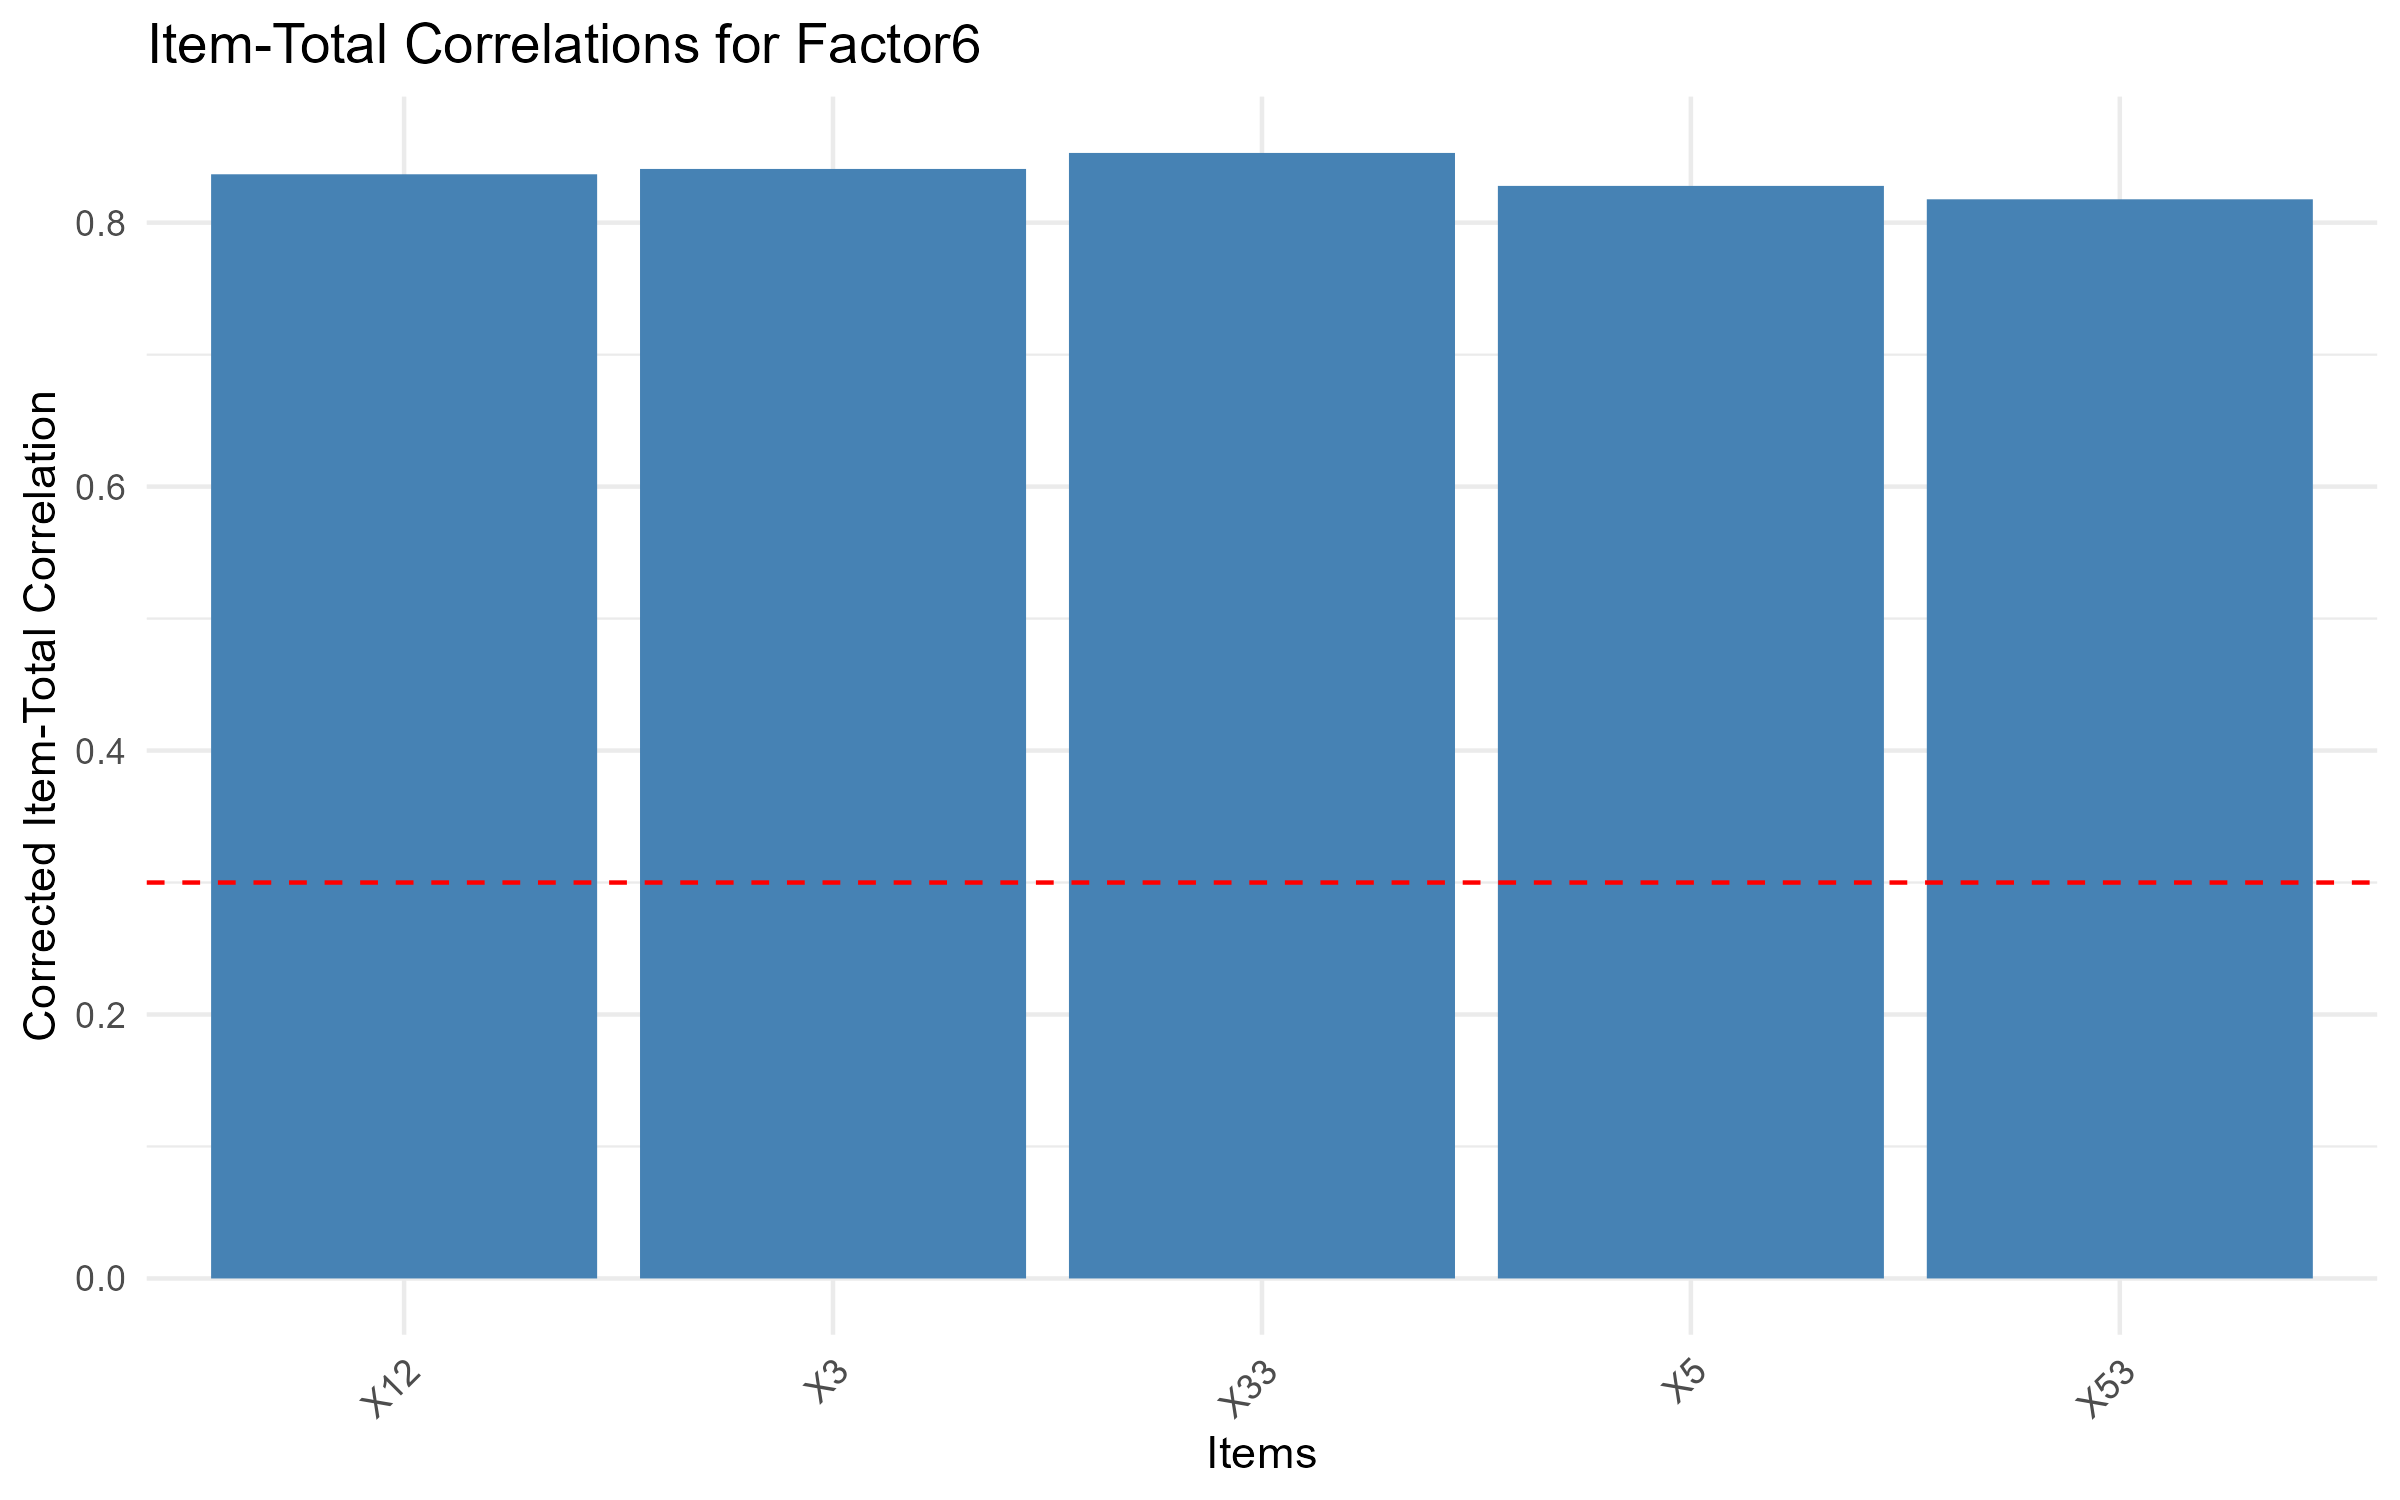
\includegraphics[width=\linewidth]{../../assets/images/reliability_Factor6.png}
        \caption{Độ tin cậy Factor 6}
        \label{fig:reliability_f6}
    \end{subfigure}
    \hfill
    \begin{subfigure}[b]{0.45\linewidth}
        \centering
        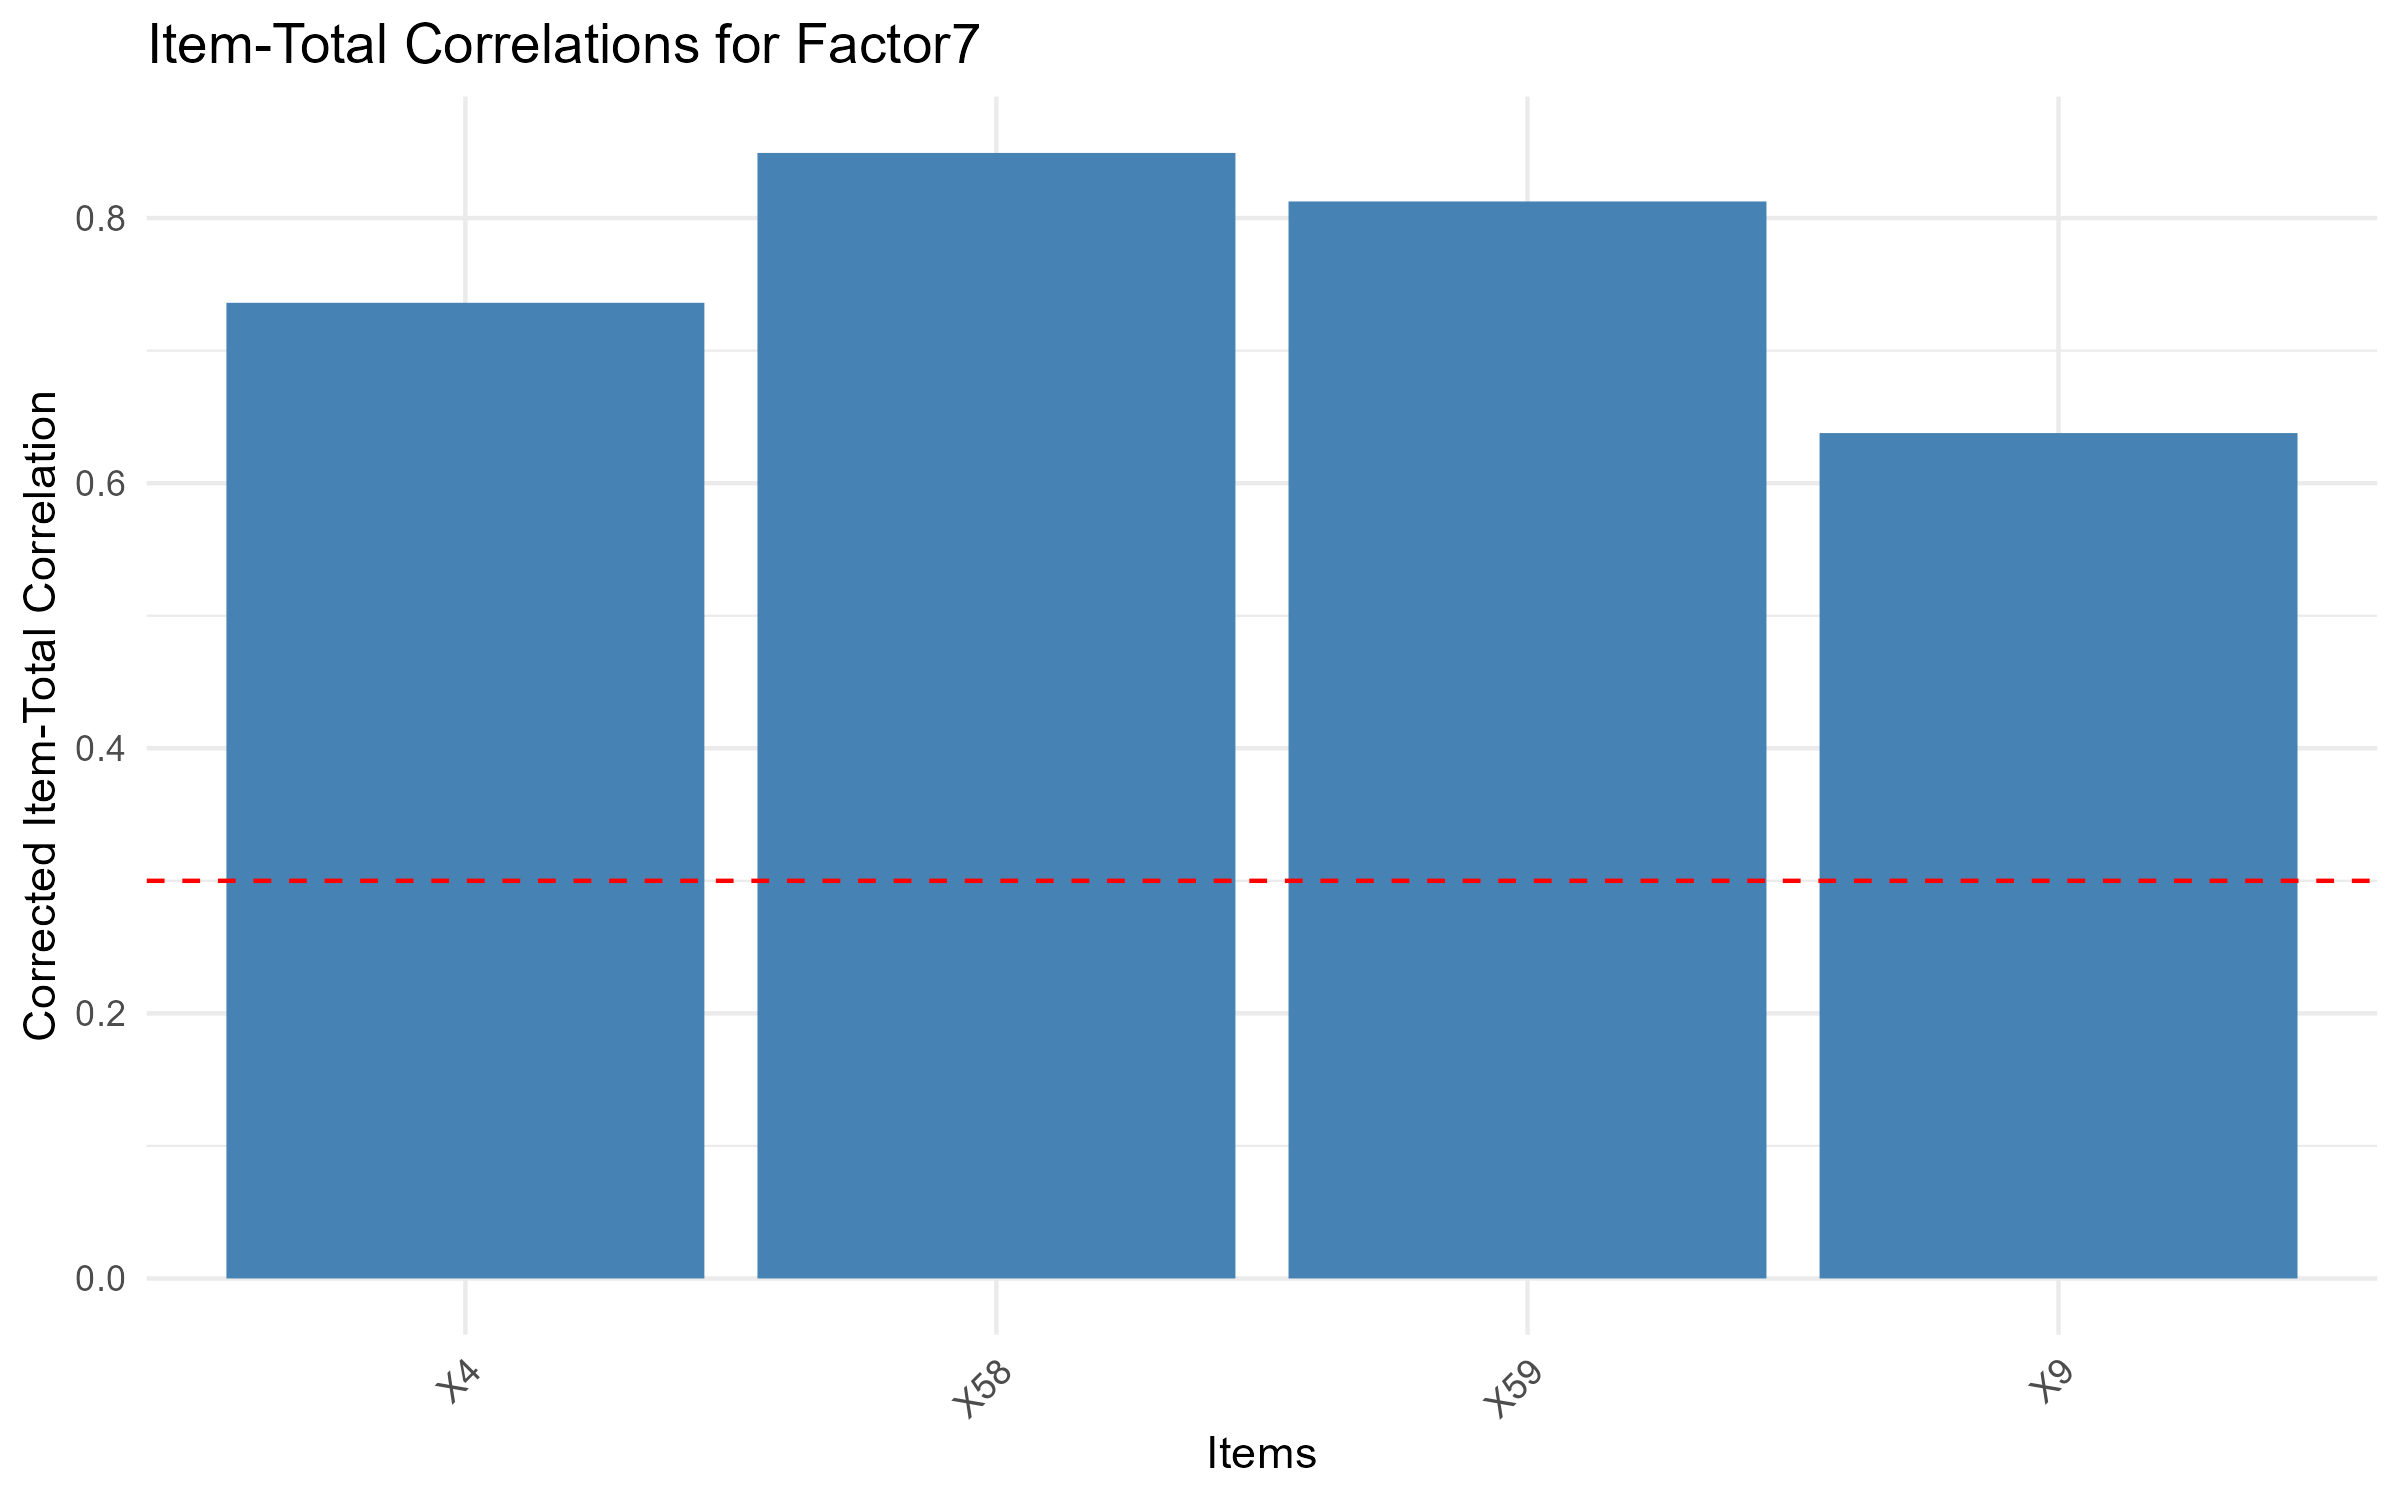
\includegraphics[width=\linewidth]{../../assets/images/reliability_Factor7.png}
        \caption{Độ tin cậy Factor 7}
        \label{fig:reliability_f7}
    \end{subfigure}

    \caption{Biểu đồ độ tin cậy từng nhân tố}
    \label{fig:efa_reliability}
\end{figure}

\subsection{Quy trình phân tích tổng hợp}

\subsection{Đánh giá hiệu quả mô hình}
\subsubsection*{Cross-validation cho PCA}
Đánh giá tính ổn định của các thành phần chính thông qua validation chéo.

\subsubsection*{Metrics cho clustering}
\begin{itemize}
    \item \textbf{Silhouette coefficient}: $s_i = \frac{b_i - a_i}{\max(a_i, b_i)}$
    \item \textbf{Calinski-Harabasz index}: $\frac{SS_B/(k-1)}{SS_W/(n-k)}$
    \item \textbf{Davies-Bouldin index}: $\frac{1}{k}\sum_{i=1}^k \max_{j \neq i} \frac{\sigma_i + \sigma_j}{d_{ij}}$
\end{itemize}

Quy trình phân tích dữ liệu nhiều chiều tổng hợp bao gồm nhiều bước từ khám phá dữ liệu ban đầu đến xây dựng mô hình cuối cùng. Mỗi kỹ thuật có ưu điểm riêng và cần được lựa chọn phù hợp với mục tiêu nghiên cứu cụ thể. Việc kết hợp nhiều phương pháp thường cho kết quả toàn diện và đáng tin cậy hơn.

\section{Phân tích nhân tố khám phá (EFA)}

EFA là một kỹ thuật thống kê được sử dụng để xác định cấu trúc ẩn trong một tập dữ liệu với nhiều biến quan sát \cite{vu2022, hair2019, tabachnick2019}.

\subsection{Mô hình phân tích nhân tố}

Mô hình EFA tương tự như mô hình factor analysis đã trình bày, nhưng tập trung vào việc khám phá số lượng và bản chất của các nhân tố mà không có giả định trước về cấu trúc.

\subsection{Kiểm định độ tin cậy Cronbach's Alpha}

Cronbach's Alpha là một thước đo độ tin cậy nội bộ của thang đo, đánh giá mức độ nhất quán giữa các mục trong cùng một nhân tố. Giá trị Alpha từ 0.7 trở lên được coi là chấp nhận được.

\section{Kết luận chương}

Chương này đã trình bày một cách hệ thống các phương pháp phân tích dữ liệu nhiều chiều quan trọng. Những điểm chính cần ghi nhớ:

\begin{itemize}
    \item \textbf{PCA} phù hợp cho giảm chiều và trực quan hóa dữ liệu
    \item \textbf{Factor Analysis} tập trung vào tìm cấu trúc tiềm ẩn trong dữ liệu quan sát
    \item \textbf{EFA} giúp khám phá số lượng và bản chất của các nhân tố ẩn
    \item Đánh giá độ tin cậy bằng Cronbach's Alpha để đảm bảo tính nhất quán nội bộ
    \item Việc kết hợp nhiều phương pháp thường cho hiểu biết sâu sắc hơn về dữ liệu
    \item Cần validation kỹ lưỡng để đảm bảo tính tin cậy của kết quả
\end{itemize}

Các kỹ thuật này tạo thành nền tảng vững chắc cho việc phân tích dữ liệu phức tạp, từ nghiên cứu khoa học đến các ứng dụng thực tiễn trong nhiều lĩnh vực khác nhau.